\documentclass[letter,graphicx]{beamer}



\mode<presentation>
{
  \usetheme{Warsaw}
  % or ...

  \setbeamercovered{transparent}
  % or whatever (possibly just delete it)
}


\usepackage[english]{babel}
% or whatever

\usepackage[latin1]{inputenc}
% or whatever
\usepackage{verbatim}
\usepackage{times}
\usepackage[T1]{fontenc}
\usepackage{mychicago}
\renewcommand{\citeN}{\shortciteN}
% Or whatever. Note that the encoding and the font should match. If T1
% does not look nice, try deleting the line with the fontenc.

\logo{\includegraphics[width=.1\textwidth]{./images/official_NOAA_logo.pdf}}

\title[microhaplotypes from NGS] % (optional, use only with long paper titles)
{Reaching haplotopia: the promise and practice \\
of short-read microhaplotypes\\
in molecular ecology}

\subtitle{} % (optional)

\author[Eric C. Anderson] % (optional, use only with lots of authors)
{Eric C.~Anderson and the NMFS-SWFSC-MEGA Team}
% - Use the \inst{?} command only if the authors have different
%   affiliation.

\institute[NOAA Fisheries] % (optional, but mostly needed)
{\mbox{}
%Fisheries Ecology Division \\ Southwest Fisheries Science Center \\ Santa Cruz, CA \\ USA
\hfill
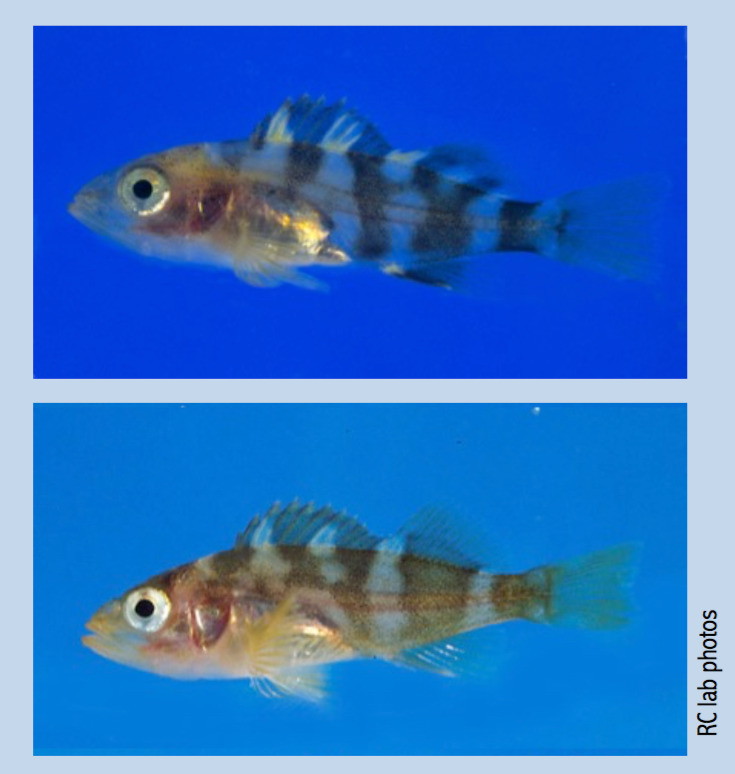
\includegraphics[height=.25\textwidth]{./mhap_figs/juvie_rockfish.png}
\hfill
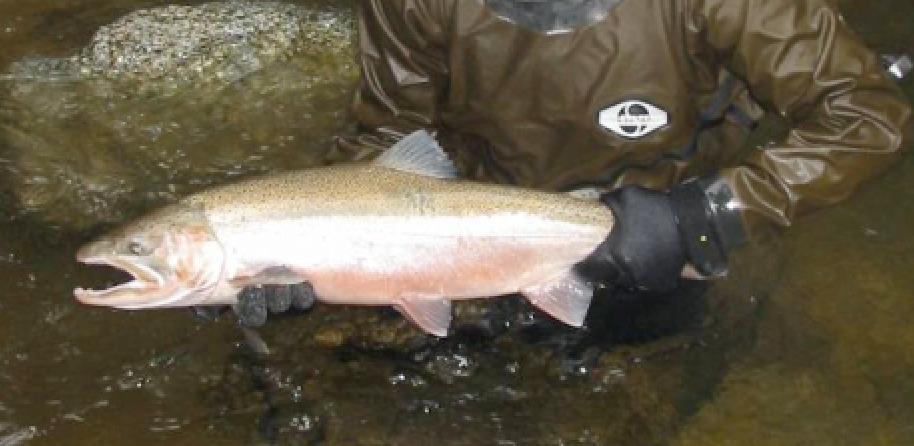
\includegraphics[height=.25\textwidth]{./mhap_figs/steelhead.png}
\hfill\mbox{}
}
% - Use the \inst command only if there are several affiliations.
% - Keep it simple, no one is interested in your street address.

\date[Durham 2016] % (optional)
{
Durham University Ecology Seminar\\ 14 NOV 2016}

\subject{Talks}


%% More eric commands for inserting some small figures
\newcommand{\smikid}{\includegraphics[width=3.7ex]{images/smiley_blue_kid.pdf}}
\newcommand{\smired}{\includegraphics[width=2.9ex]{images/smiley_sad_red.png}}
\newcommand{\smiblue}{\includegraphics[width=2.9ex]{images/smiley_happy_blue.png}}
\newcommand{\thh}{^\mathrm{th}}
\newcommand{\tc}{\textcolor}
\def\bm#1{\mathpalette\bmstyle{#1}}
\def\bmstyle#1#2{\mbox{\boldmath$#1#2$}}


\begin{document}




\begin{frame}
  \titlepage
\end{frame}



\begin{frame}{Collaborators and Acknowledgments}
\begin{columns}
\begin{column}{0.6\textwidth}
NOAA/SWFSC/UCSC
\begin{itemize}
\item Carlos Garza
\item Anthony Clemento
\item Thomas Ng (UCSC grad student)
\item Diana Baetscher (UCSC grad student)
\end{itemize}
\end{column}


\begin{column}{0.4\textwidth}
UCSC Rockfish Project:
\begin{itemize}
\item Mark Carr
\item Chris Edwards
\item Dan Malone
\item Emily Saarman
\item Patrick Drake
\item Anna Lowe 
\end{itemize}
{\centering 

\includegraphics[width=0.7\textwidth]{mhap_figs/nsf.jpg}
}
\end{column}
\end{columns}
\end{frame}

%	Chris Edwards <cedwards@ucsc.edu>,
%Mark Carr <mhcarr@ucsc.edu>,
%John Carlos Garza <carlos.garza@noaa.gov>,
%"Eric C. Anderson" <eric.anderson@noaa.gov>,
%Emily Saarman <esaarman@ucsc.edu>,
%Daniel Malone <dmalone@ucsc.edu>,
%Patrick Drake <pdrake@ucsc.edu>,
%Anna Lowe <ablowe@ucsc.edu>
% Thomas Ng
% Diana Baetscher
%


\begin{frame}{Overview}
\begin{itemize}
\item Next Generation Sequencing Methods
\begin{itemize}
\item sequencing, assembly, alignment
\item genome representation reduction
\item amplicon sequencing
\end{itemize}

\item Microhaplotypes
\begin{itemize}
\item available by reanalysis of most data sets
\item advantages
\end{itemize}

\item Example problem: Dispersal of larval rockfish
\begin{itemize}
\item parentage and sibling inference in a multispecies context
\end{itemize}

\item Tools from our lab:
\begin{itemize}
\item CKMRsim
\item haPLOType
\end{itemize}

\end{itemize}
\end{frame}







\begin{frame}{Next Generation Sequencing -- I}
\framesubtitle{Illumina Sequencing By Synthesis}
{\centering
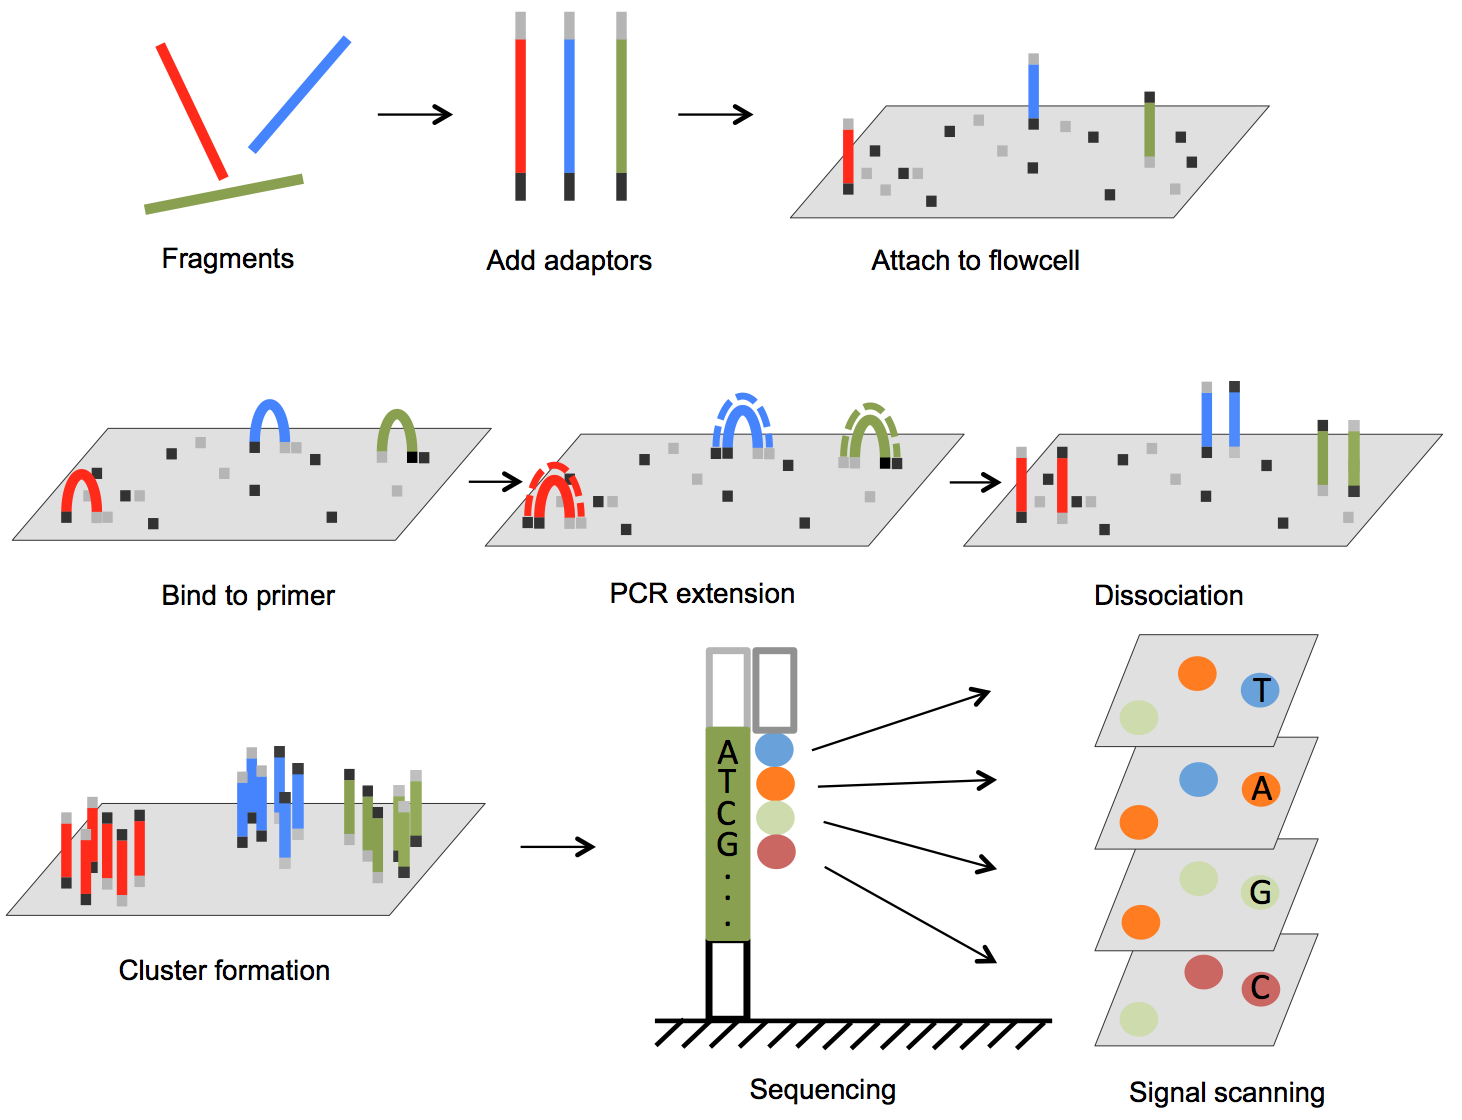
\includegraphics[height=0.80\textheight]{mhap_figs/illumina_fig.png}
}\\
{\tiny http://www.intechopen.com}
\end{frame}







\begin{frame}{Next Generation Sequencing -- II}
\framesubtitle{{\em de novo} ``genome'' assembly}
{\centering
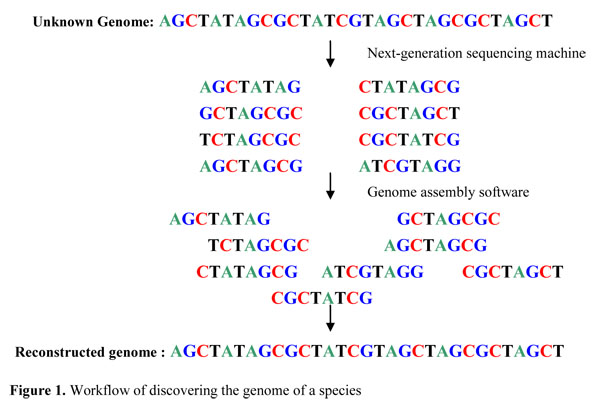
\includegraphics[height=0.75\textheight]{mhap_figs/assembly.png}
}\\
{\tiny http://www.cs.hku.hk}
\end{frame}






\begin{frame}{Next Generation Sequencing -- III}
\framesubtitle{Alignment of sequencing reads to ``genome'' allows \\
identification of polymorphisms and genotyping}
{\centering
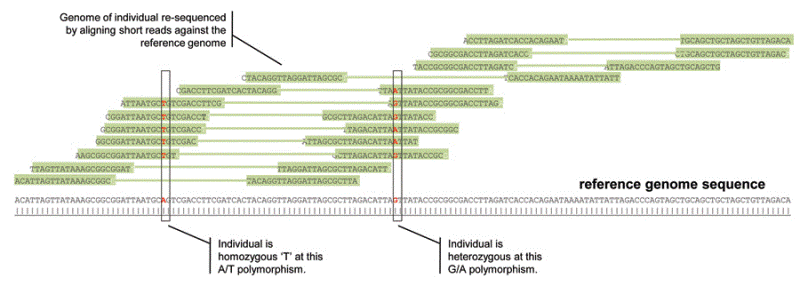
\includegraphics[width=0.95\textwidth]{mhap_figs/alignment.png}
}\\
{\tiny http://www.historyofnimr.org.uk}
\end{frame}






\begin{frame}{Sequencing Capacities}
\framesubtitle{Continually increasing.  Examples from Illumina:}
\begin{itemize}
\item Small Benchtop MiSeq sequencer:
\begin{itemize}
\item 25 million reads/run ($\approx \$1,000$ reagent cost)
\item up to 2 x 300 bp
\end{itemize}

\item Large Core facility HiSeq sequencer:
\begin{itemize}
\item 500 million reads per lane ($\approx \$3,400$)
\item up to 2 x 150 bp
\end{itemize}
\end{itemize}


\begin{itemize}
\item {\em Many} individuals can be sequenced together via combinatorial barcoding.
\end{itemize}
\end{frame}





\begin{frame}{Combinatorial Barcodes}
$\bullet$ Imagine that you prepared individuals in batches (plates) of three at time.\\
$\bullet$ Individual barcode on one end; plate barcode on the other.
\begin{center}
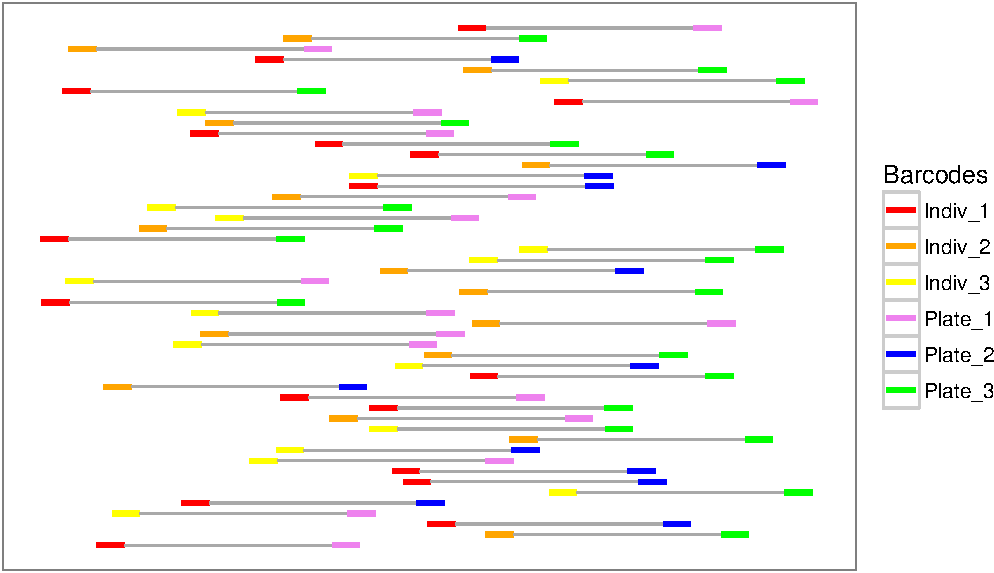
\includegraphics[width=.95\textwidth]{mhap_figs/combi-barcodes-crop.pdf}
\end{center}
\end{frame}






\begin{frame}{Fundamental Tradeoff}
\begin{itemize}
\item Accurate determination of the sequence {\em at a genomic position} and {\em in an individual} requires a sufficient number of reads sequencing that position in that individual.
\item So, either:
\begin{itemize}
\item One (or a few) individuals across large swaths of genome
\item Many individuals across a reduced portion of the genome
\end{itemize}
\item Methods for {\em reduced representation} sequencing:
\begin{itemize}
\item RNAseq (sequence just the transcriptome)
\item RADseq (Restriction Associated DNA sequencing)
\item GBS (Genotyping by Sequencing)
\item Capture/Bait methods (MyBaits, RAPTURE, etc.)
\item Amplicon Sequencing (GTseq)
\end{itemize}
\end{itemize}
\end{frame}





\begin{frame}{GTseq amplicon sequencing}
\begin{center}
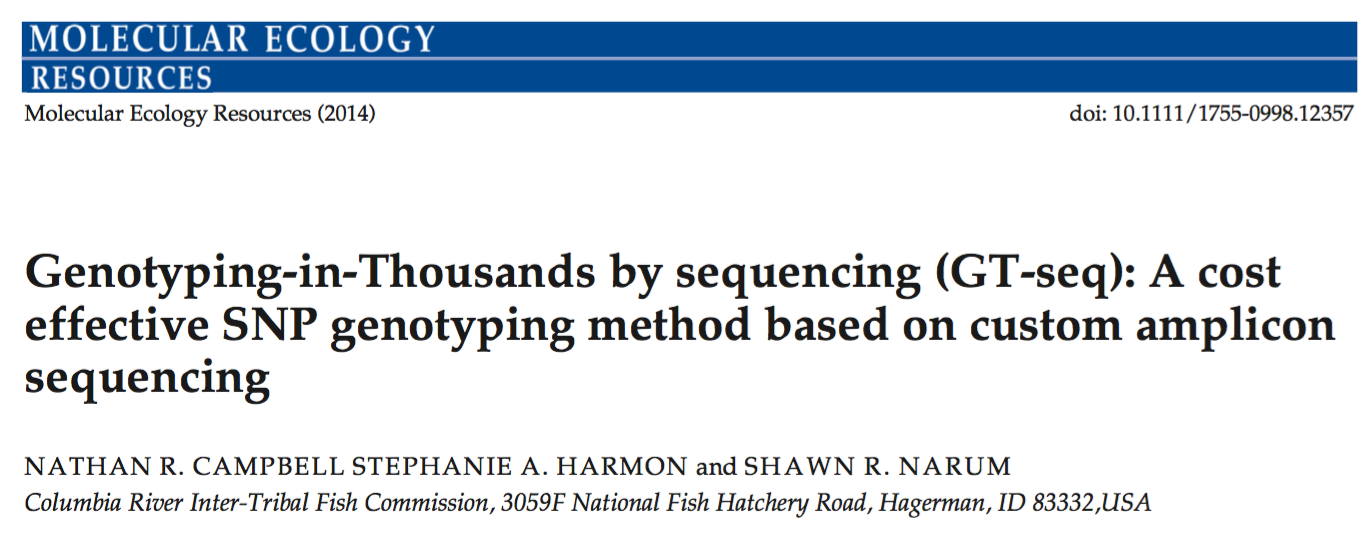
\includegraphics[width=0.95\textwidth]{mhap_figs/gtseq-header.png}
\end{center}
\begin{itemize}
\item Multiplexed PCR primers amplify regions of interest.
\item Amplicon sequencing of 200--500 regions in 500--2,000 individuals
\item $\approx \$7$/individual
\item Converted Fluidigm SNP assays.  Tens of 1,000s of salmon each year.
\end{itemize}
\end{frame}








\begin{frame}{GTseq -- I {\small (coming off the sequencer\ldots)}}
\framesubtitle{2 Amplicons; 3 individuals on each of 3 plates (9 individuals total)}
\begin{center}
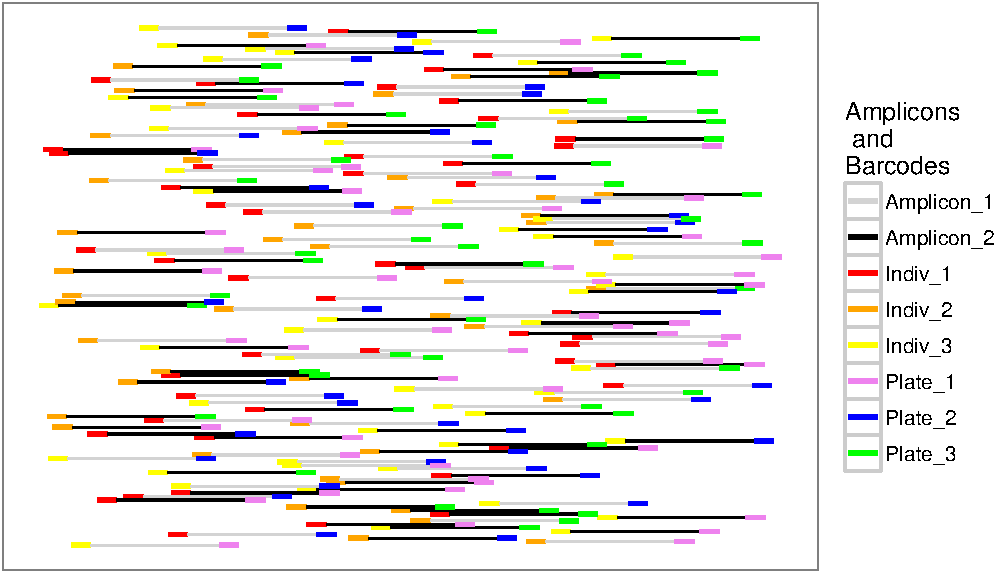
\includegraphics[width=0.95\textwidth]{mhap_figs/gtseq-soup-crop.pdf}
\end{center}
\end{frame}





\begin{frame}{GTseq -- II (aligned amplicons)}
\framesubtitle{Amplicon sequences are known. Alignment {\em in silico} is straightforward.}
\begin{center}
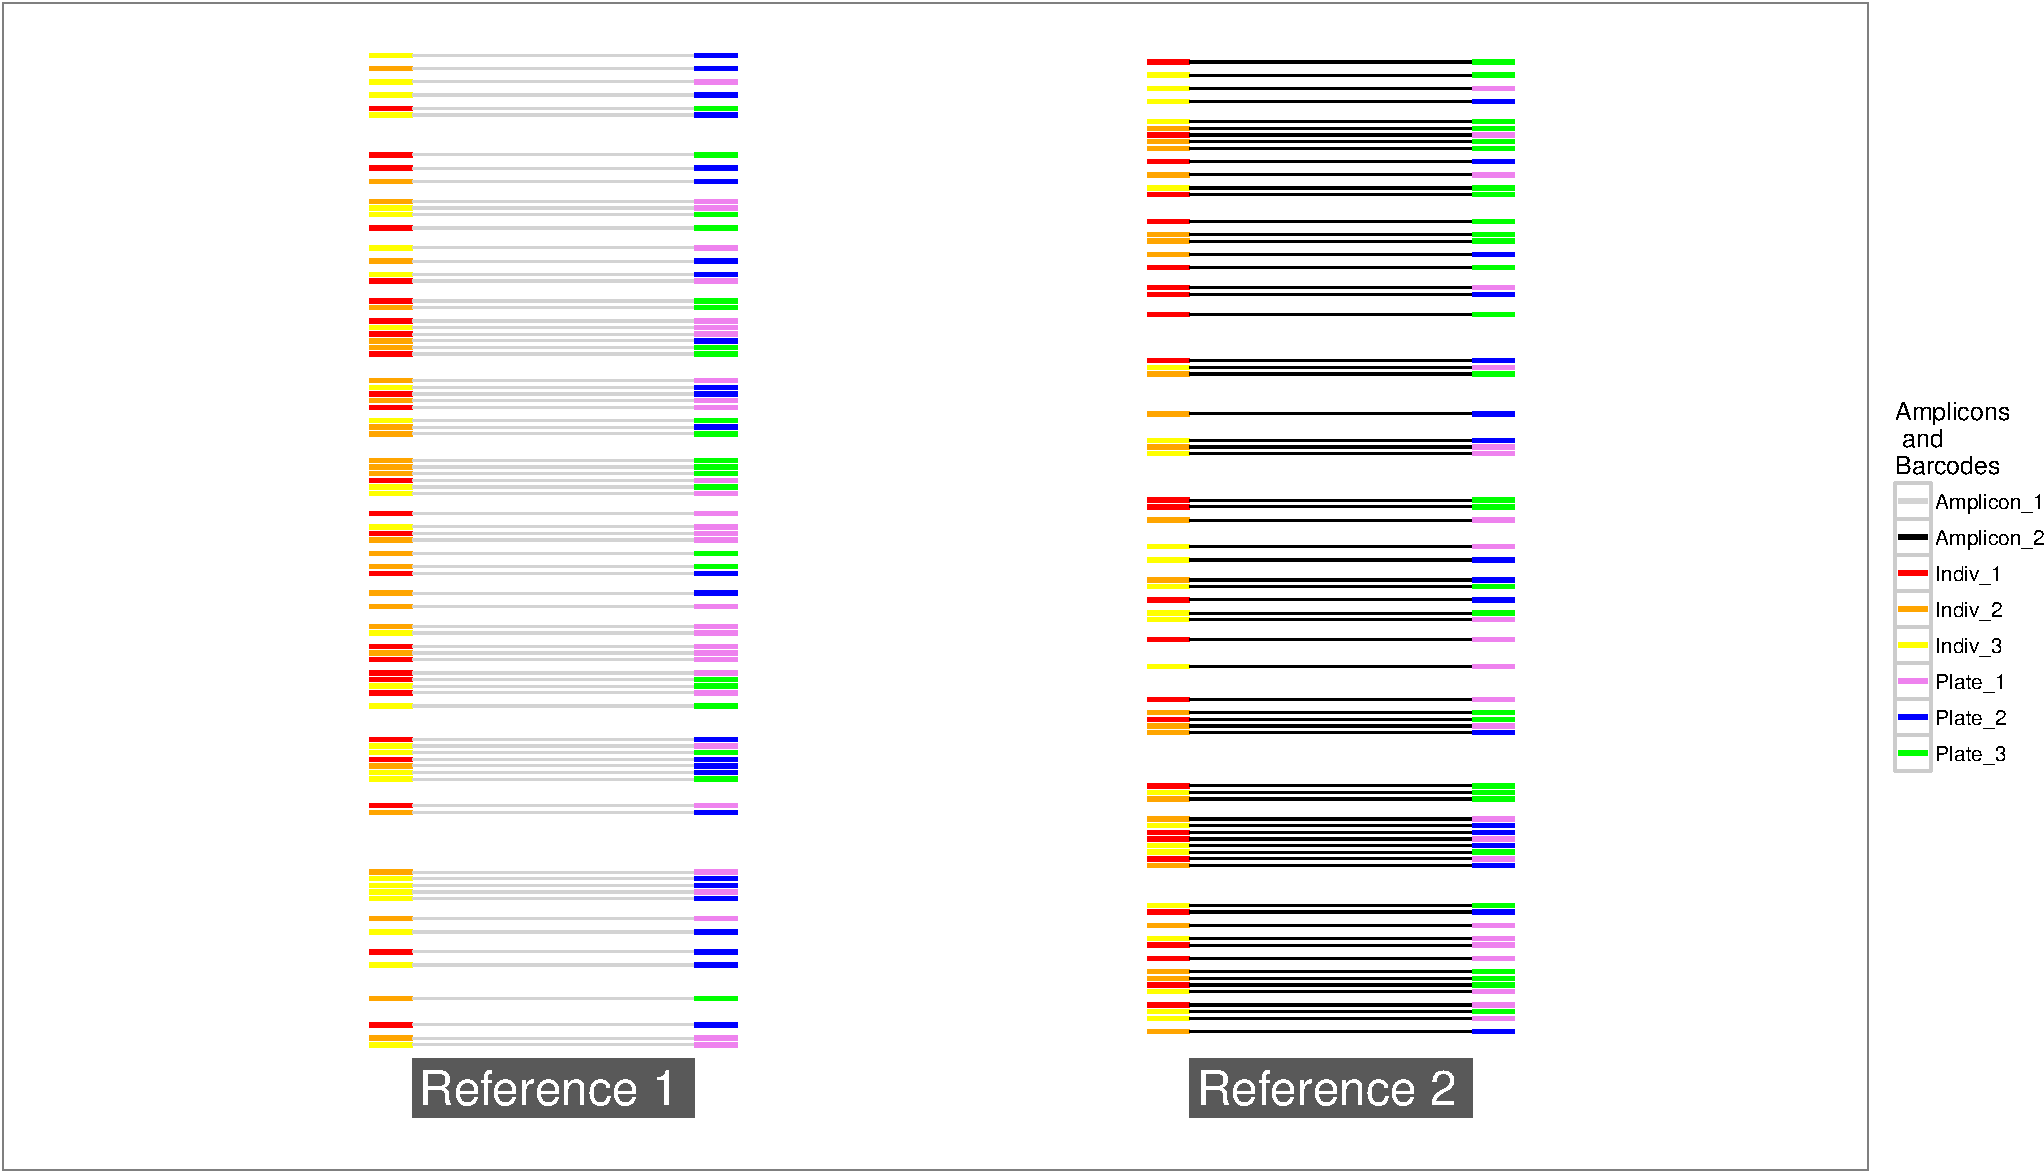
\includegraphics[width=0.95\textwidth]{mhap_figs/gtseq-amps-crop.pdf}
\end{center}
\end{frame}



\begin{frame}{GTseq -- III (``demultiplexing'')}
\framesubtitle{Identify individual origin of reads via combinatorial barcodes}
\begin{center}
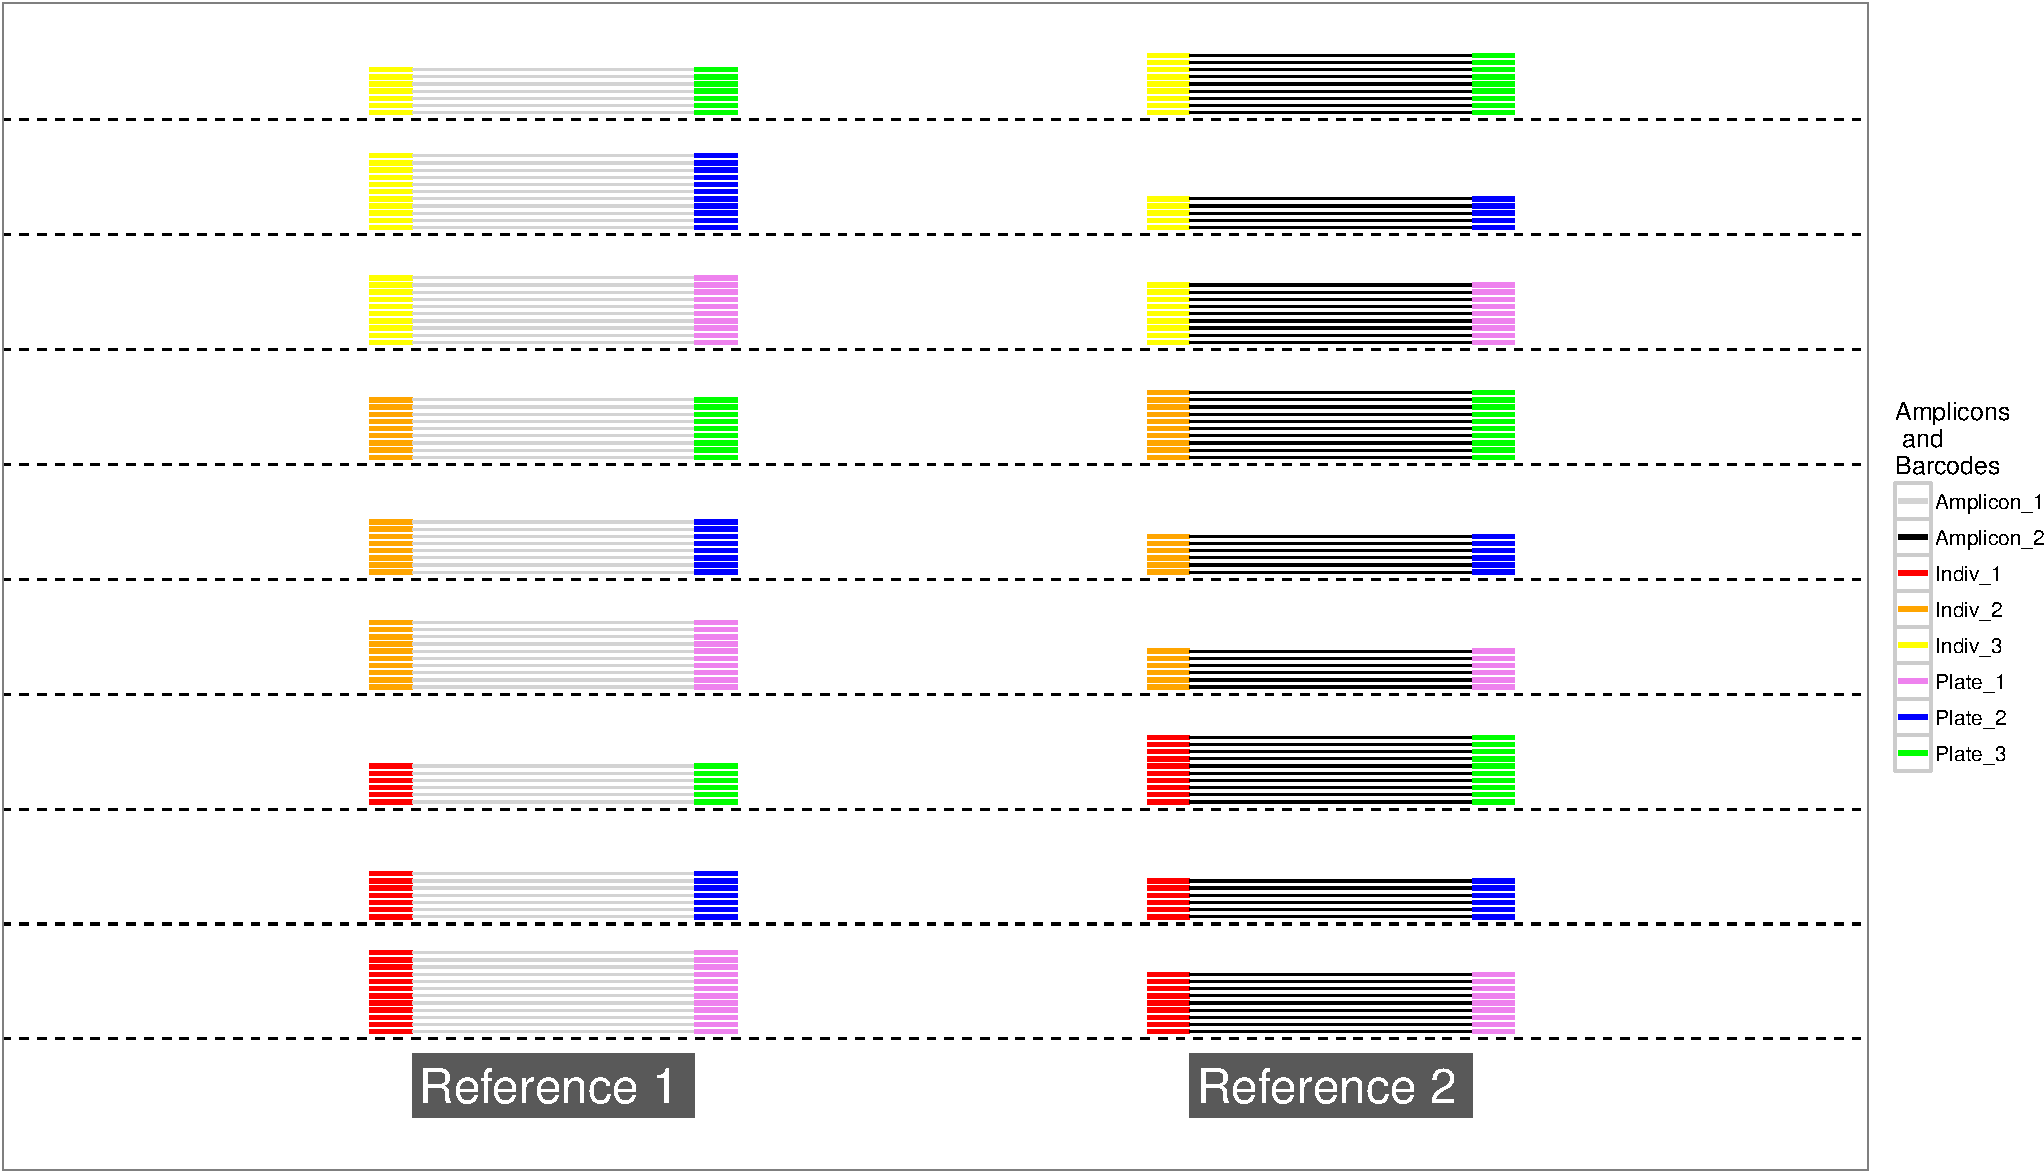
\includegraphics[width=0.95\textwidth]{mhap_figs/gtseq-demultiplexed-crop.pdf}
\end{center}
\end{frame}





\begin{frame}{GTseq -- IV (identify SNPs in sequence)}
\framesubtitle{Variants are easy to identify}
\begin{center}
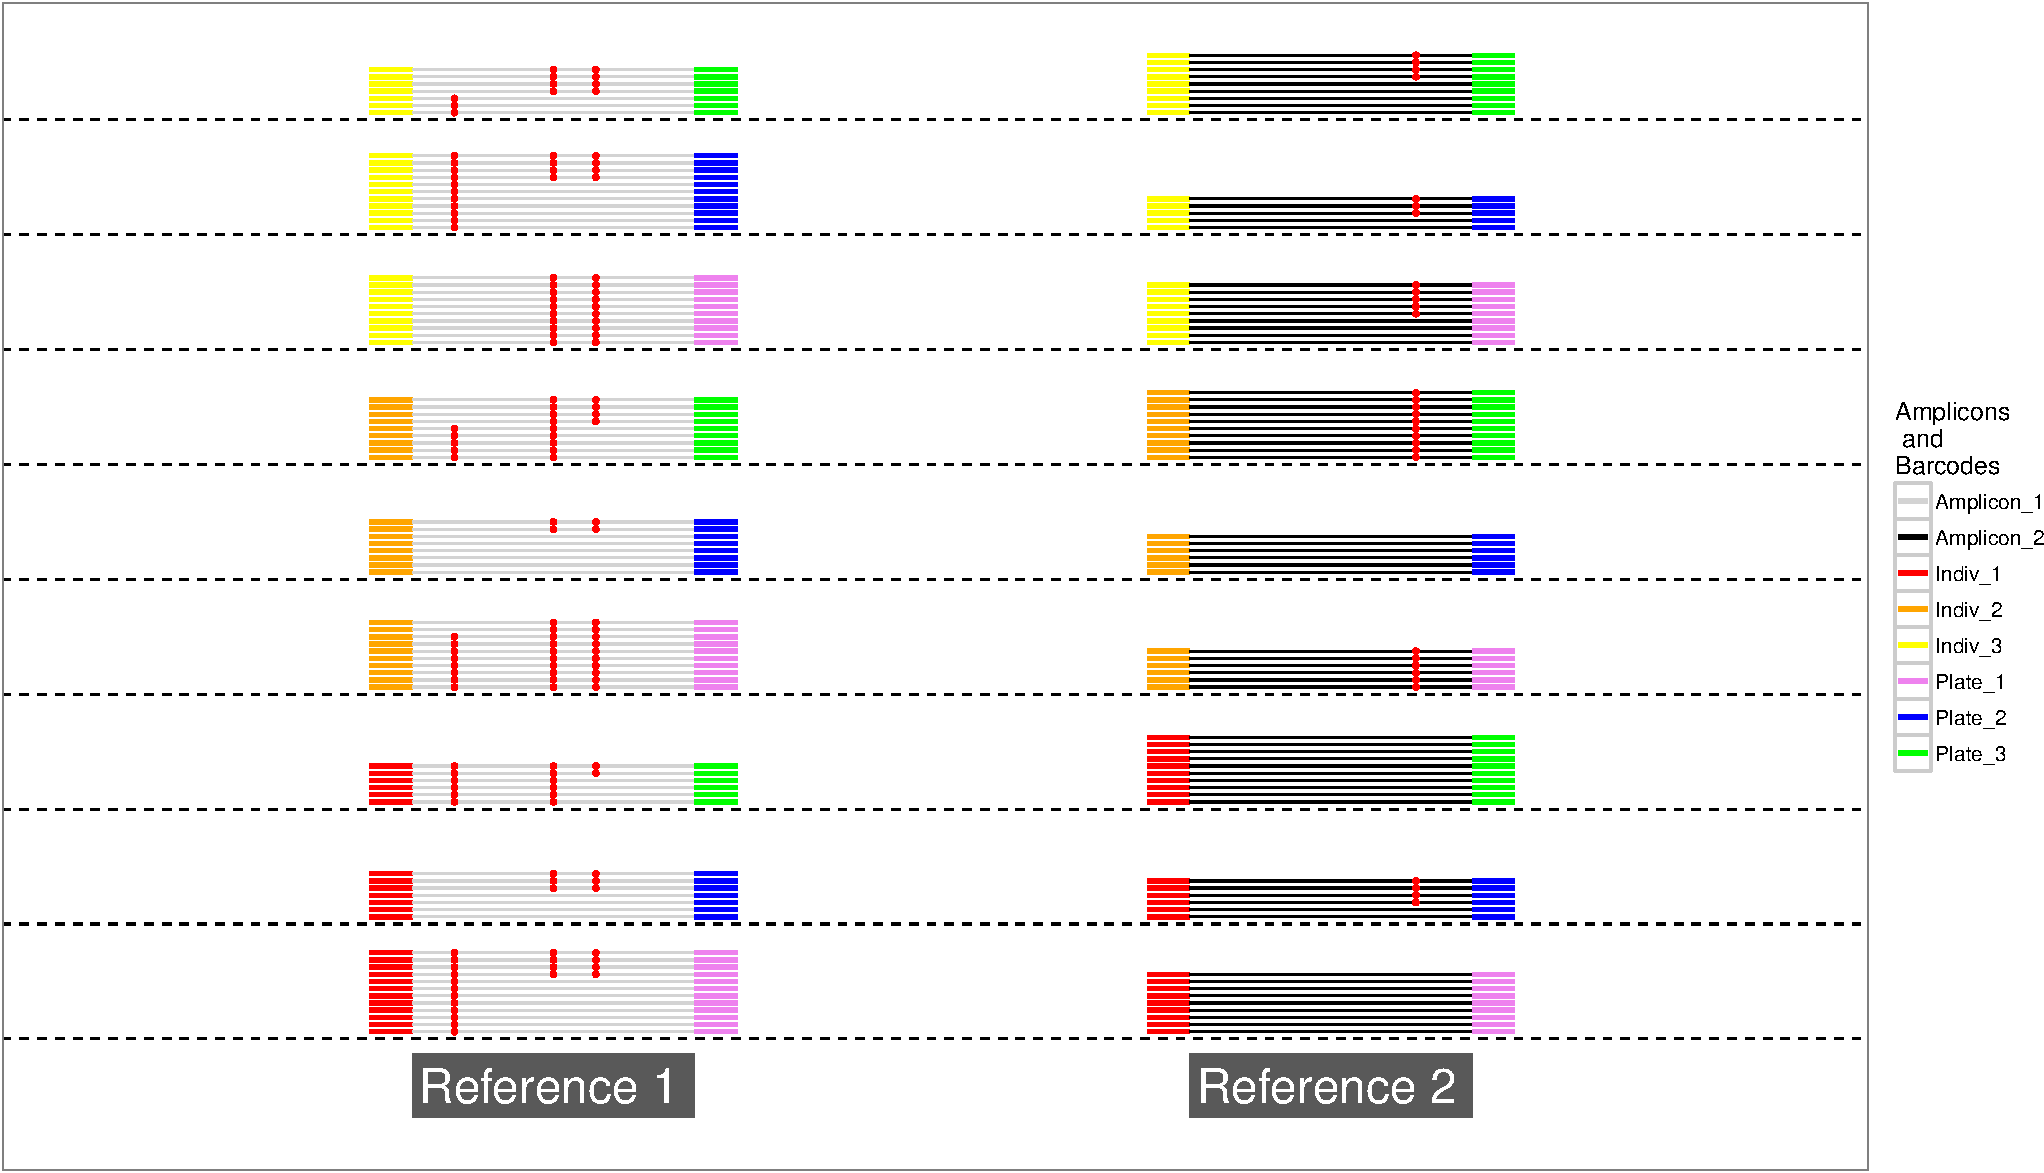
\includegraphics[width=0.95\textwidth]{mhap_figs/gtseq-snps-crop.pdf}
\end{center}
\end{frame}




\begin{frame}{Multiple SNPs in amplicons/sequences\ldots}
\framesubtitle{\ldots are almost universally ignored }
\begin{itemize}
\item Multiple SNPs in each amplicon/RAD-locus are typically scored
\item But then either:
\begin{enumerate}
\item Only a single SNP from each amplicon/locus is used
\item OR, all SNPs are treated as unlinked
\end{enumerate}
Depending on the analyses, the result is either a lack of power or (potentially) incorrect inference.
\end{itemize}
\end{frame}






\begin{frame}{Phase of SNPs on reads is almost universally ignored}
\begin{center}
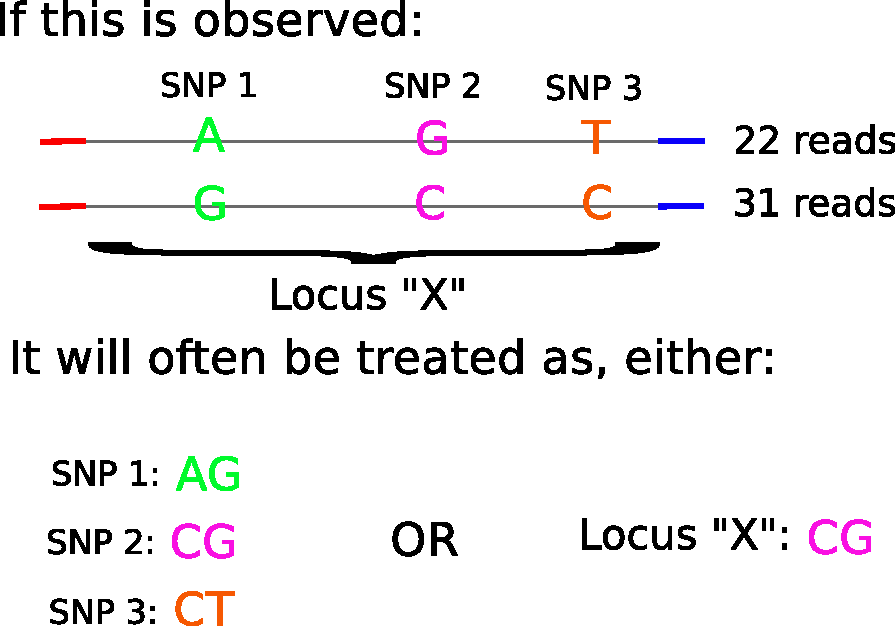
\includegraphics[width=0.94\textwidth]{mhap_figs/three-snp-reads.pdf}
\end{center}
\end{frame}













\begin{frame}{Microhaplotypes}
\framesubtitle{A simple idea / plea, that\ldots}
\begin{center}
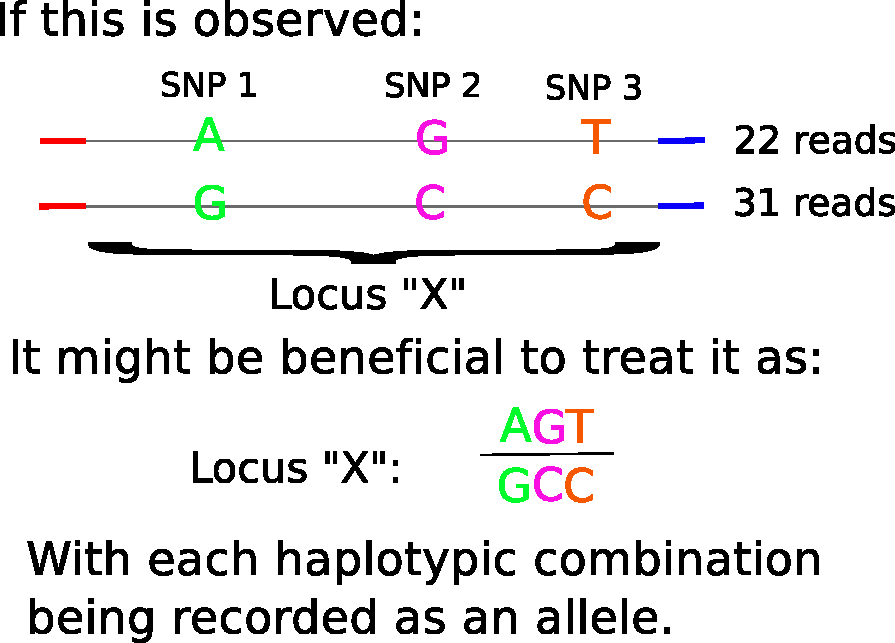
\includegraphics[width=0.94\textwidth]{mhap_figs/three-snp-reads-mhap.pdf}
\end{center}
\end{frame}






\begin{frame}{Microhaplotypes}
\framesubtitle{Potential advantages}
\begin{itemize}
\item Multiallelic loci
\begin{itemize}
\item More power for relationship inference / pedigree reconstruction
\end{itemize}
\item Need not discard SNPs from certain loci
\begin{itemize}
\item Retain low-frequency variants.  Useful for population structure in recently diverged populations.
\end{itemize}
\item Amplicons typically cross-amplify between closely-related species
\begin{itemize}
\item Unlike single SNP assays, the microhaplotype data collection method, unmodified,
can yield useful data for non-target species.
\end{itemize}
\end{itemize}
\end{frame}







\begin{frame}{Marine Population Structure}
\begin{columns}
\begin{column}{0.45\textwidth}
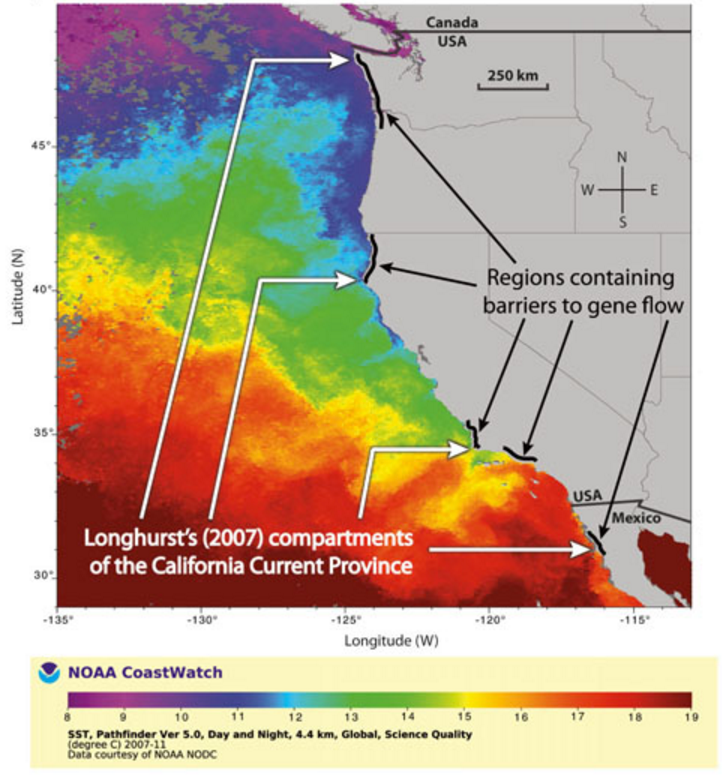
\includegraphics[width=1.1\textwidth]{mhap_figs/vetter_coast.png}\\
{\tiny Hyde and Vetter (2009) CJFAS}
\end{column}
\begin{column}{0.55\textwidth}  %%<--- here
\begin{itemize}
\item California Current
\begin{itemize}
\item Upwelling; nutrients; long larval duration
\end{itemize}
\item Barriers to gene flow
\begin{itemize}
\item Suspected from patterns of genetic variation
\item Difficult to estimate actual migration/dispersal rates
\end{itemize}
\item Considerable interest in larval dispersal/retention
\begin{itemize}
\item Design of MPAs, etc.
\end{itemize}
\end{itemize}

\end{column}
\end{columns}
\end{frame}




\begin{frame}{Larval Dispersal off California}
\framesubtitle{Heavily influenced by Ekman transport}
\begin{columns}
\begin{column}{0.45\textwidth}
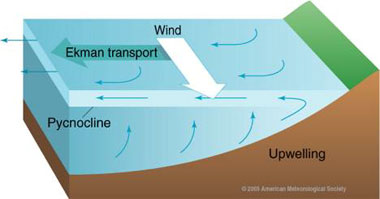
\includegraphics[width=\textwidth]{mhap_figs/ekman-upwelling.jpg}\\
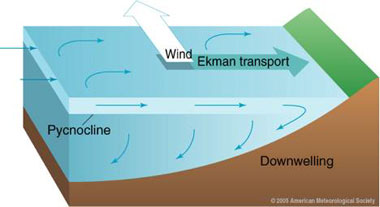
\includegraphics[width=\textwidth]{mhap_figs/ekman-downwelling.jpg}\\
{\tiny Amer. Meterol. Soc.}
\end{column}
\begin{column}{0.55\textwidth}  %%<--- here
\begin{itemize}
\item Typical Pattern:
\begin{itemize}
\item Winds blowing south down coast
\item Water transport offshore
\end{itemize}
\item Periods of relaxation:
\begin{itemize}
\item Winds blowing to the north
\item Water transport toward shore
\end{itemize}
\item Larval recruit origins
\begin{itemize}
\item Coarse current models suggest most come from far away
\item BUT, Fine-scale current irregularities might allow local
larval retention 
\end{itemize}

\end{itemize}

\end{column}
\end{columns}


\end{frame}








\begin{frame}{Question:}
\framesubtitle{What is the degree of larval self-recruitment around Carmel Bay?}
\begin{columns}
\begin{column}{0.45\textwidth}
\mbox{}\hspace*{-1ex}
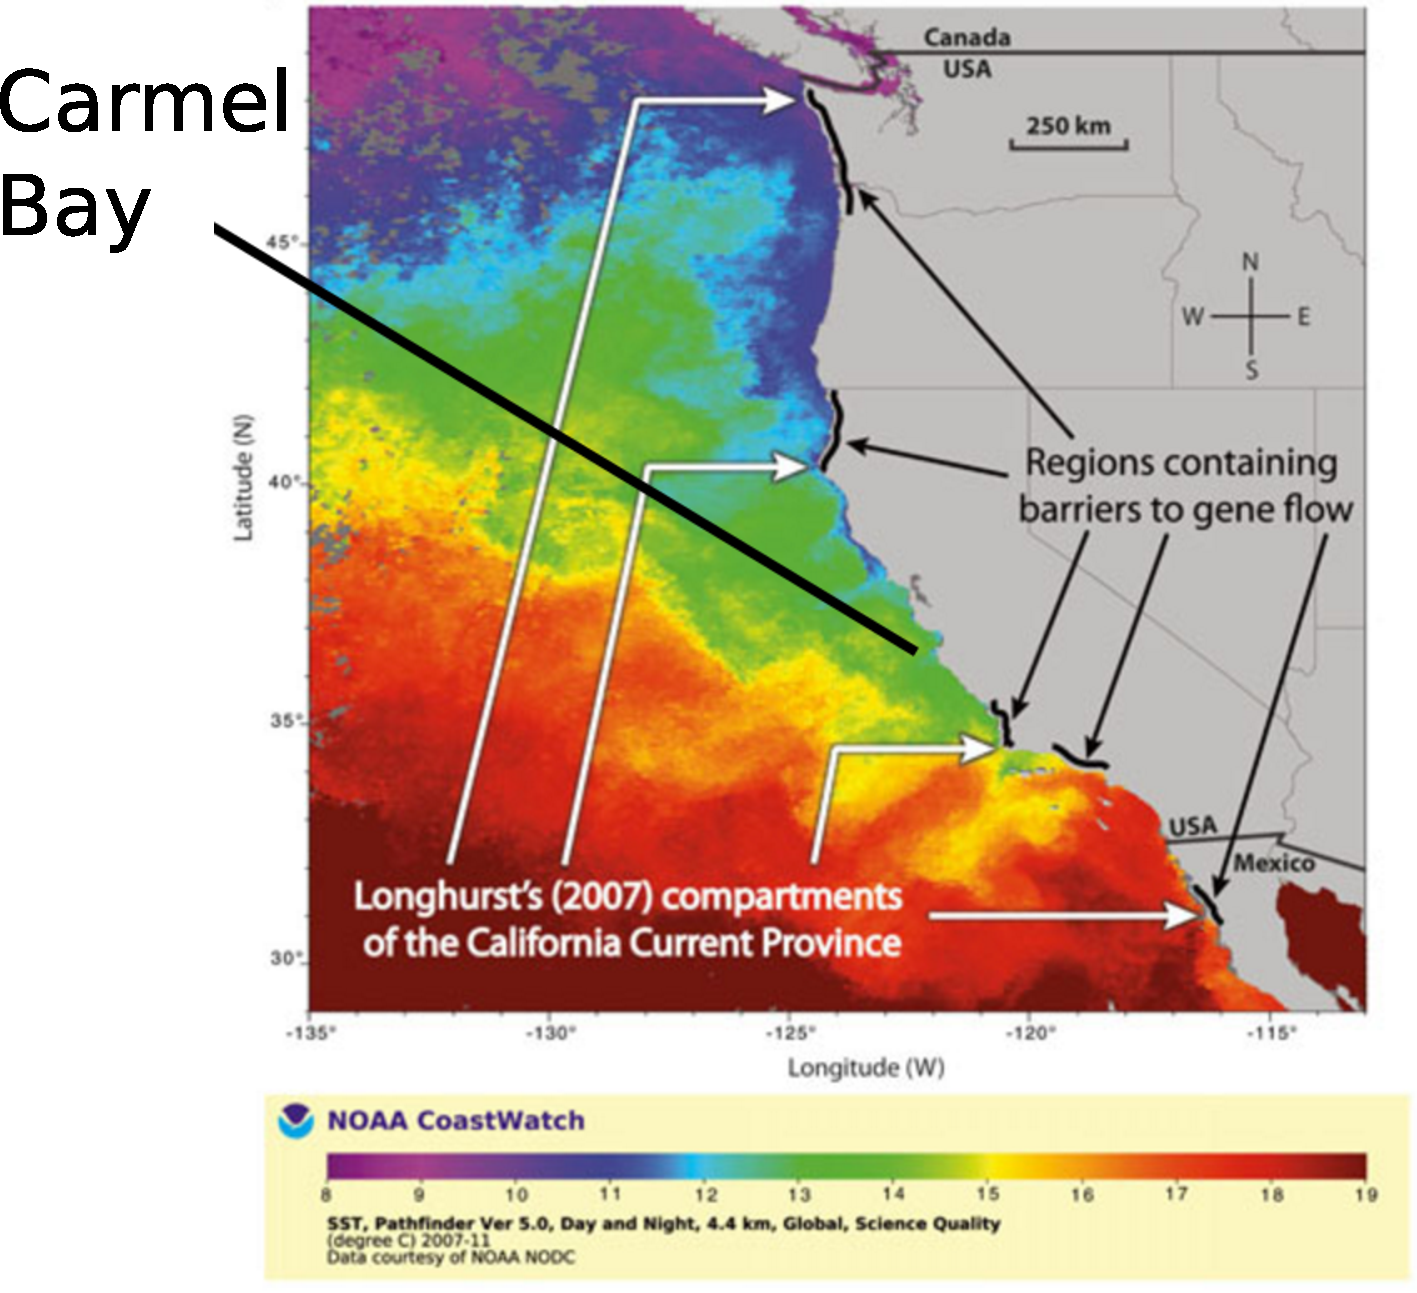
\includegraphics[width=1.2\textwidth]{mhap_figs/vetter_coast-CB.pdf}\\
{\tiny Hyde and Vetter (2009) CJFAS}
\end{column}
\begin{column}{0.55\textwidth}  %%<--- here
\begin{itemize}
\item Experimental Approach with Kelp Rockfish
\begin{enumerate}
\item Non-lethally sample a boatload ($\approx 5,000$) of adult fish
\item Genotype them
\item Collect tissues from $\approx 5,000$ larval recruits
\item Genotype them
\item Find parent-offspring pairs
\end{enumerate}
\end{itemize}
\end{column}
\end{columns}
\end{frame}











\begin{frame}{Kelp Rockfish ({\em Sebastes atrovirens})}

{\tiny photo: Wikimedia}
\includegraphics[width=0.9\textwidth]{mhap_figs/Sebastes_atrovirens.jpg}\\
Adults stationary.  Sampled by biopsy spear or hook-and-line.  Very active volunteer 
``recreational-sampling'' component. 
\end{frame}




\begin{frame}{SMURF traps}
\framesubtitle{Standard Monitoring Unit for the Recruitment of Reef Fishes}
\begin{center}
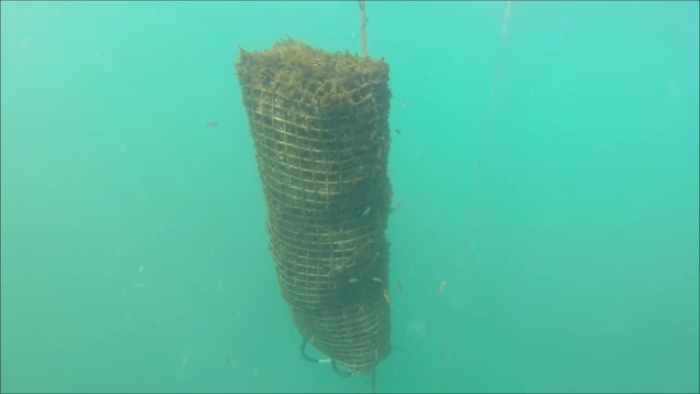
\includegraphics[width = 0.85\textwidth]{mhap_figs/smurf-solo.png}\\
{\tiny Carr-Raimondi lab photo}
\end{center}
\end{frame}



\begin{frame}{SMURF traps}
\framesubtitle{Standardized protocol for juvenile collection}
\begin{center}
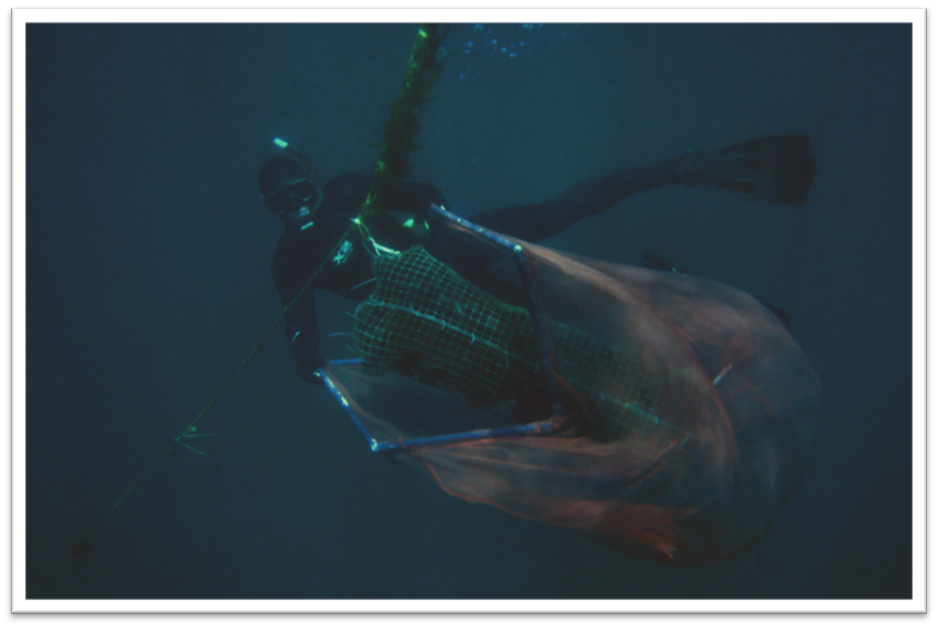
\includegraphics[width = 0.85\textwidth]{mhap_figs/smurf-binkie.png}\\
{\tiny Carr-Raimondi lab photo}
\end{center}
\end{frame}





\begin{frame}{Originally-proposed approach}
\framesubtitle{Large-scale parentage inference with microfluidic SNP assays}
\begin{center}
\mbox{}\hspace*{-.10\textwidth}
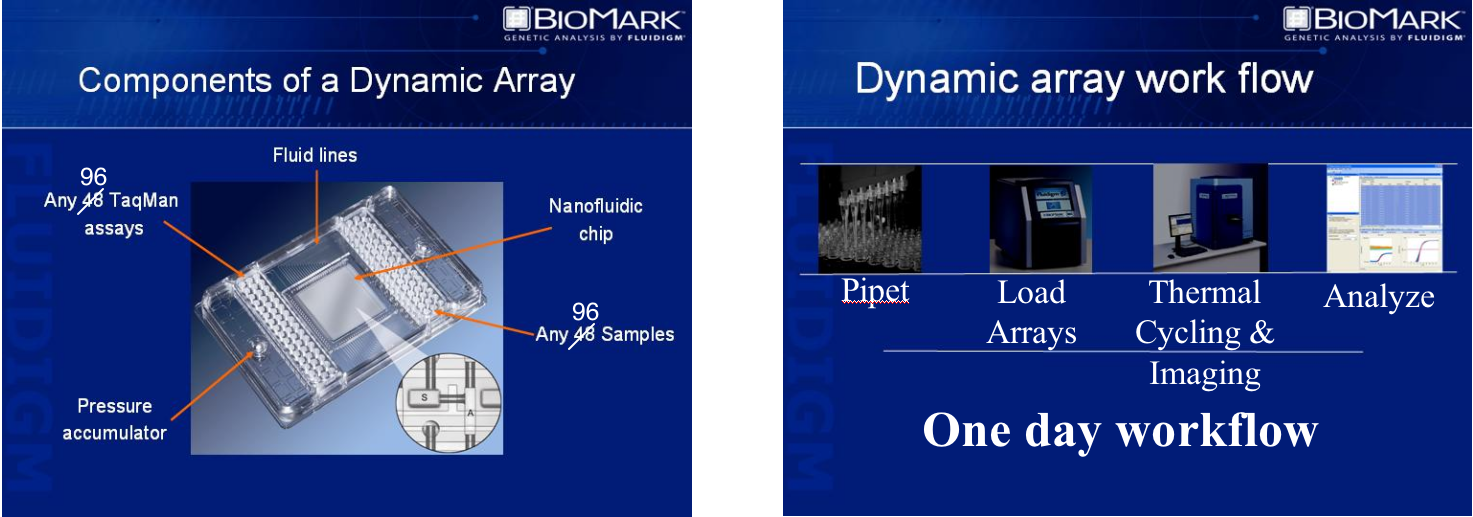
\includegraphics[width=1.16\textwidth]{mhap_figs/fluidigm.png}\\
With 96.96 Arrays and only one controller and thermal cycler, \\
can genotype almost 300 fish per day w/96 SNPs.

Cost: $<$\$15/fish 
\end{center}
\end{frame}








\begin{frame}{Nanofluidic chips, a known quantity}
\begin{center}
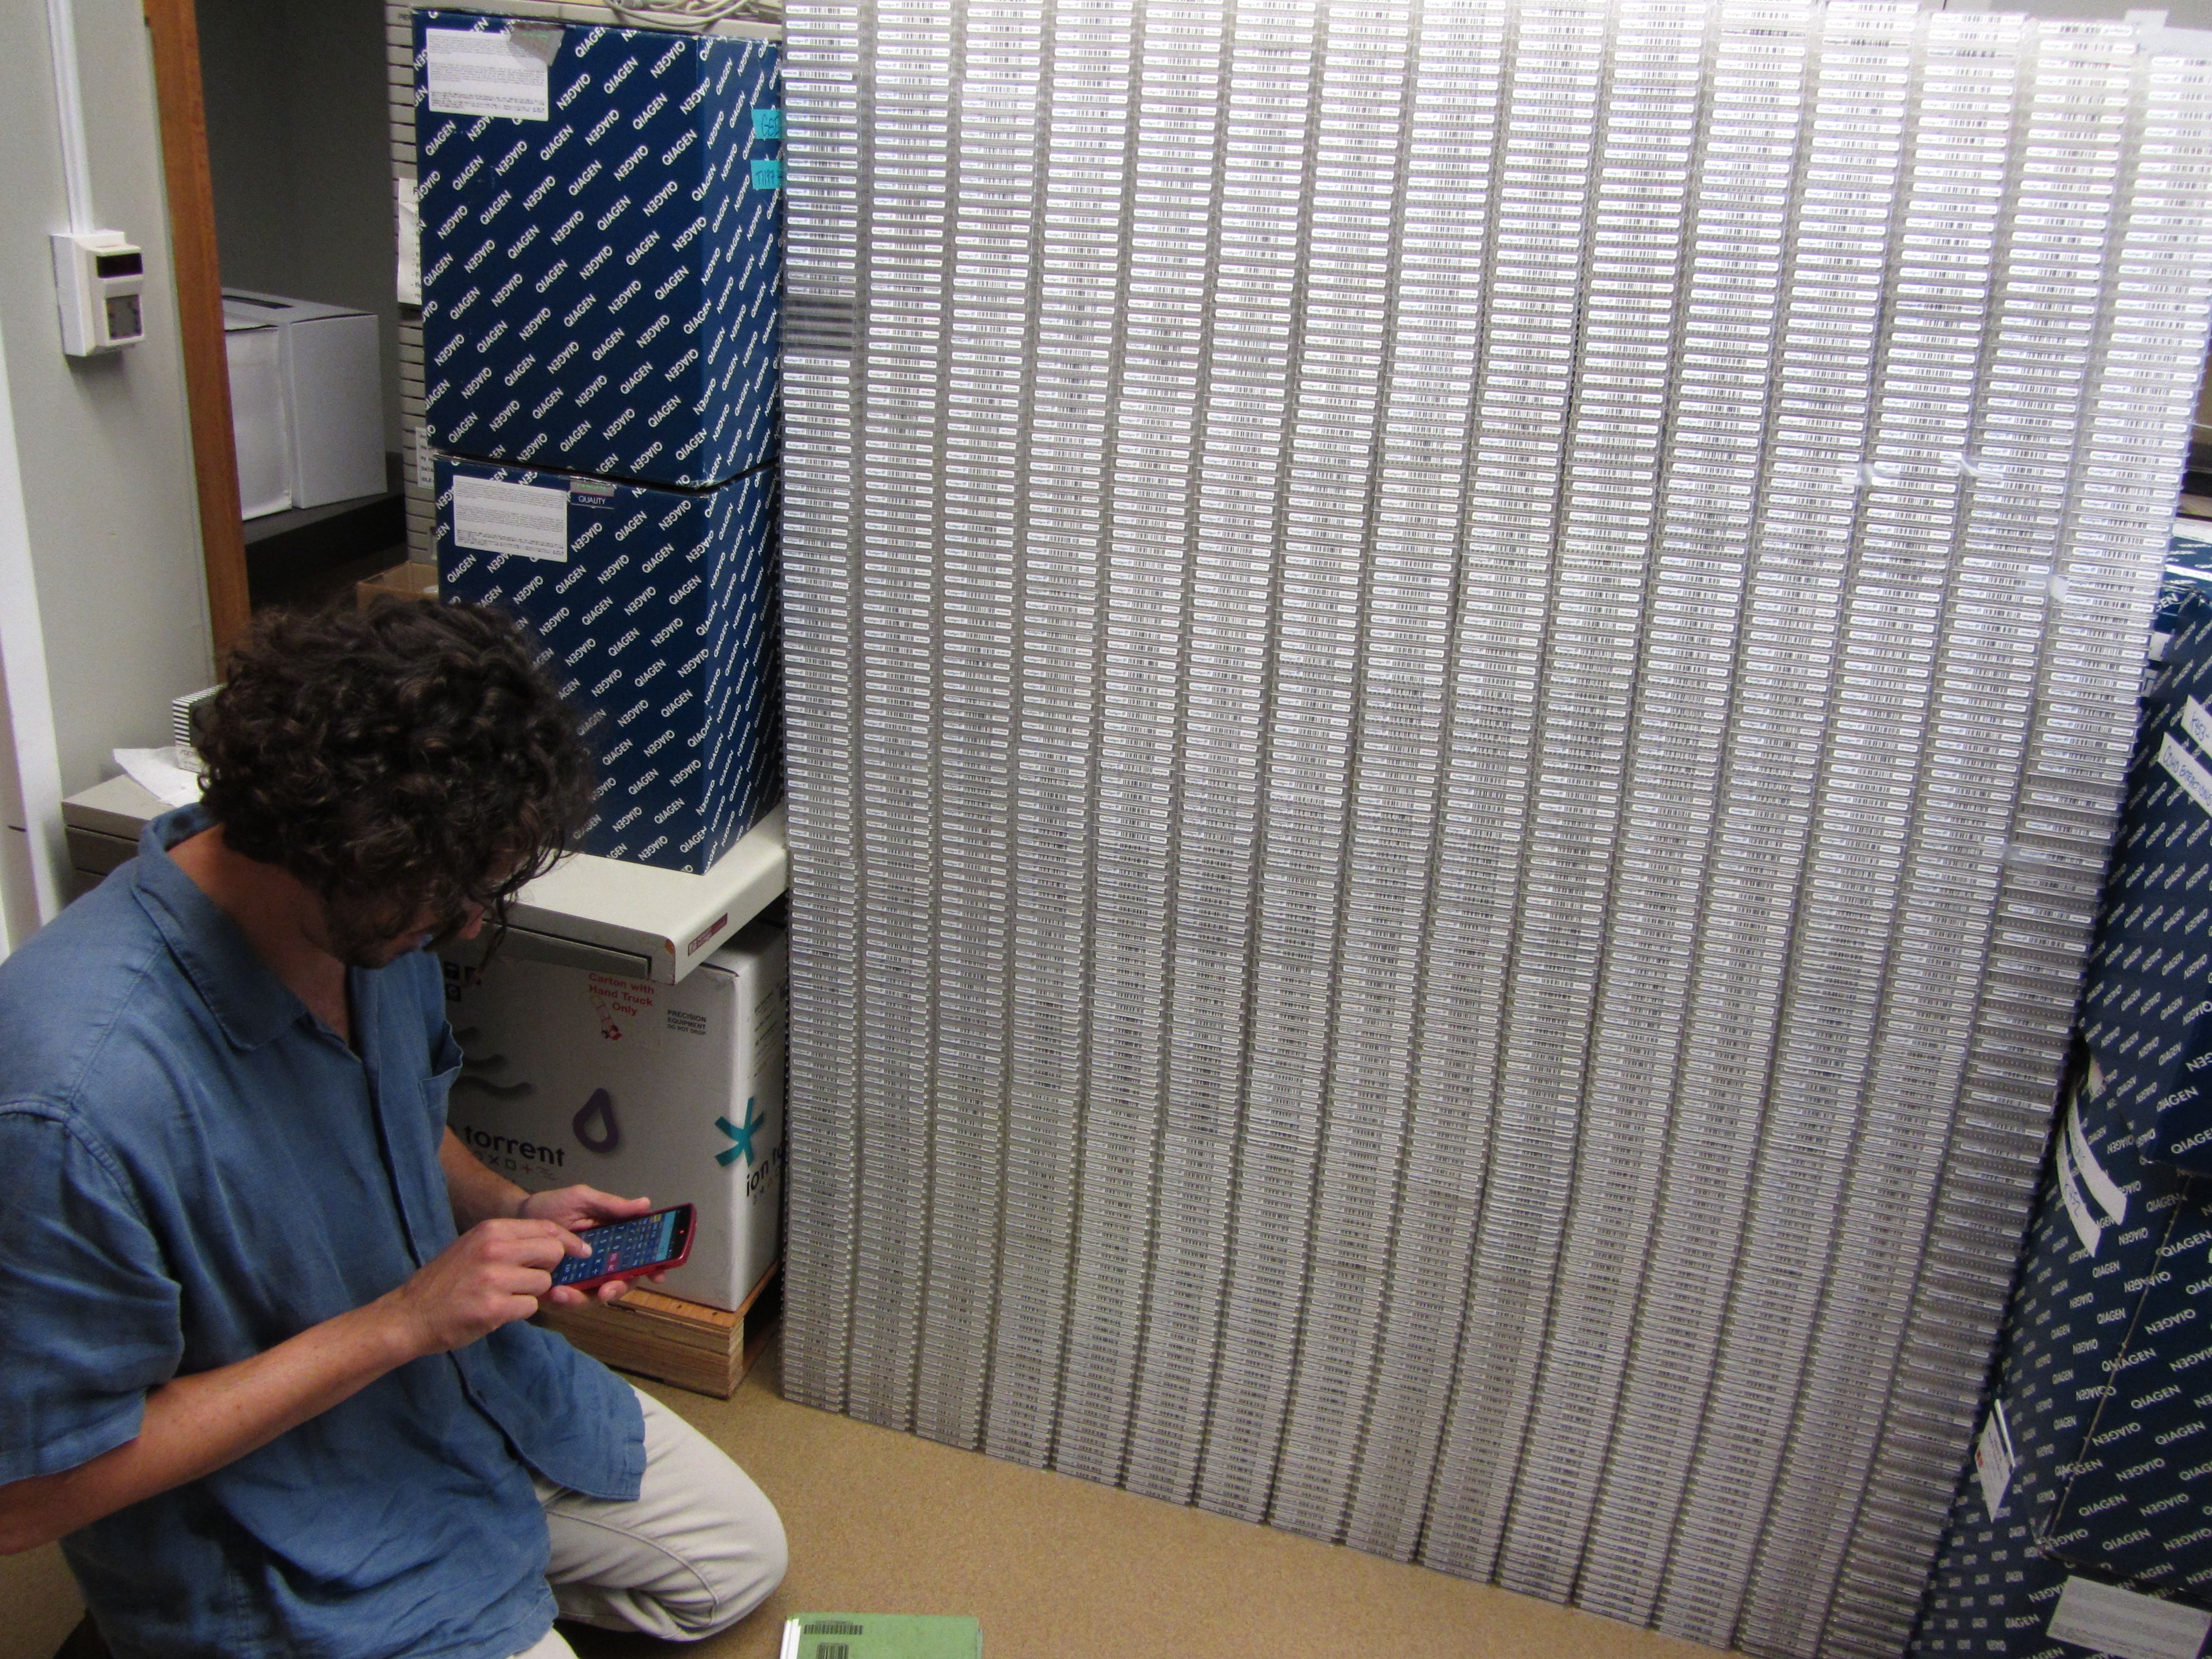
\includegraphics[width=0.75\textwidth]{mhap_figs/AC_calculating_chipwall.jpg}
\end{center}
$\bullet$ However, 96 SNPs are not enough for single parent assignments,\\
$\bullet$ and species ID in juveniles is unreliable
\end{frame}








\begin{frame}{Visual Species ID of juveniles is difficult}
\framesubtitle{Kelp, Gopher, Black-and-yellow indistinguishable at small size}
\begin{columns}
\begin{column}{0.50\textwidth}
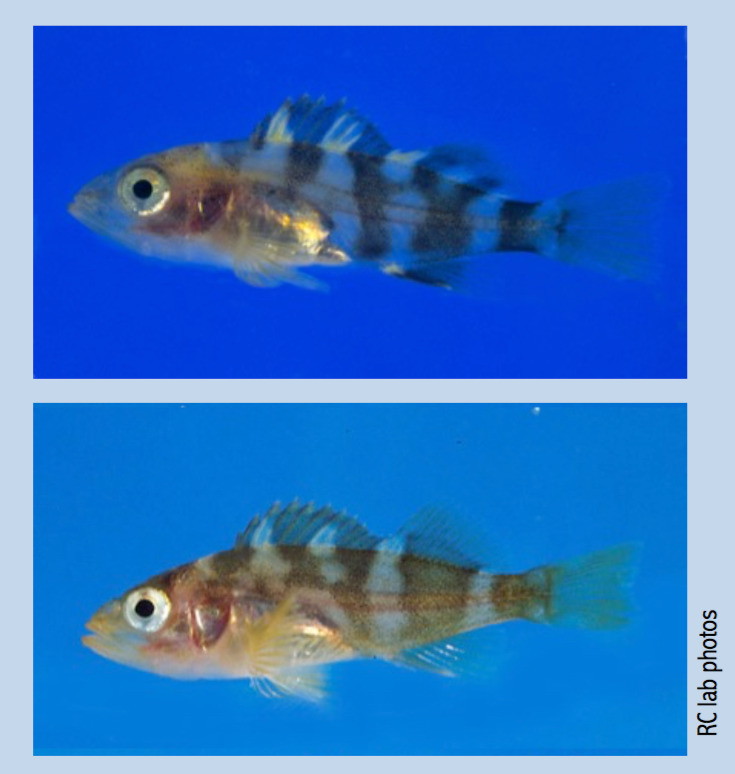
\includegraphics[width=\textwidth]{./mhap_figs/juvie_rockfish.png}
\end{column}
\begin{column}{0.50\textwidth}
\begin{itemize}
\item Up to 40\% of juvenile samples might not be kelp rockfish
\item SNP assays in non-target species tend to be monomorphic, and hence 
useless for any inference.
\item It hurts to contemplate throwing away that much
genotyping effort.
\end{itemize}
\end{column}
\end{columns}
\end{frame}










\begin{frame}{Developing GTseq Amplicons for Rockfish}
\begin{itemize}
\item ddRAD seq on 16 individuals 
\item $\approx 4,000$ genome fragments sequences
\item 200 developed into amplicons, and tested
\item 165 amplicons retained
\item Amplified and sequenced from 240 individuals.
\item Allele/Haplotype frequencies estimated
\begin{itemize}
\item 825 alleles (average of 5 haplotypes per locus)
\end{itemize}

\item Power for Parentage and Full sibling inference computed
\end{itemize}

\end{frame}
















\begin{frame}{Log-likelihood ratio distribution}
\framesubtitle{For Parent-offspring and full-sib pairs vs Unrelated}
\begin{center}
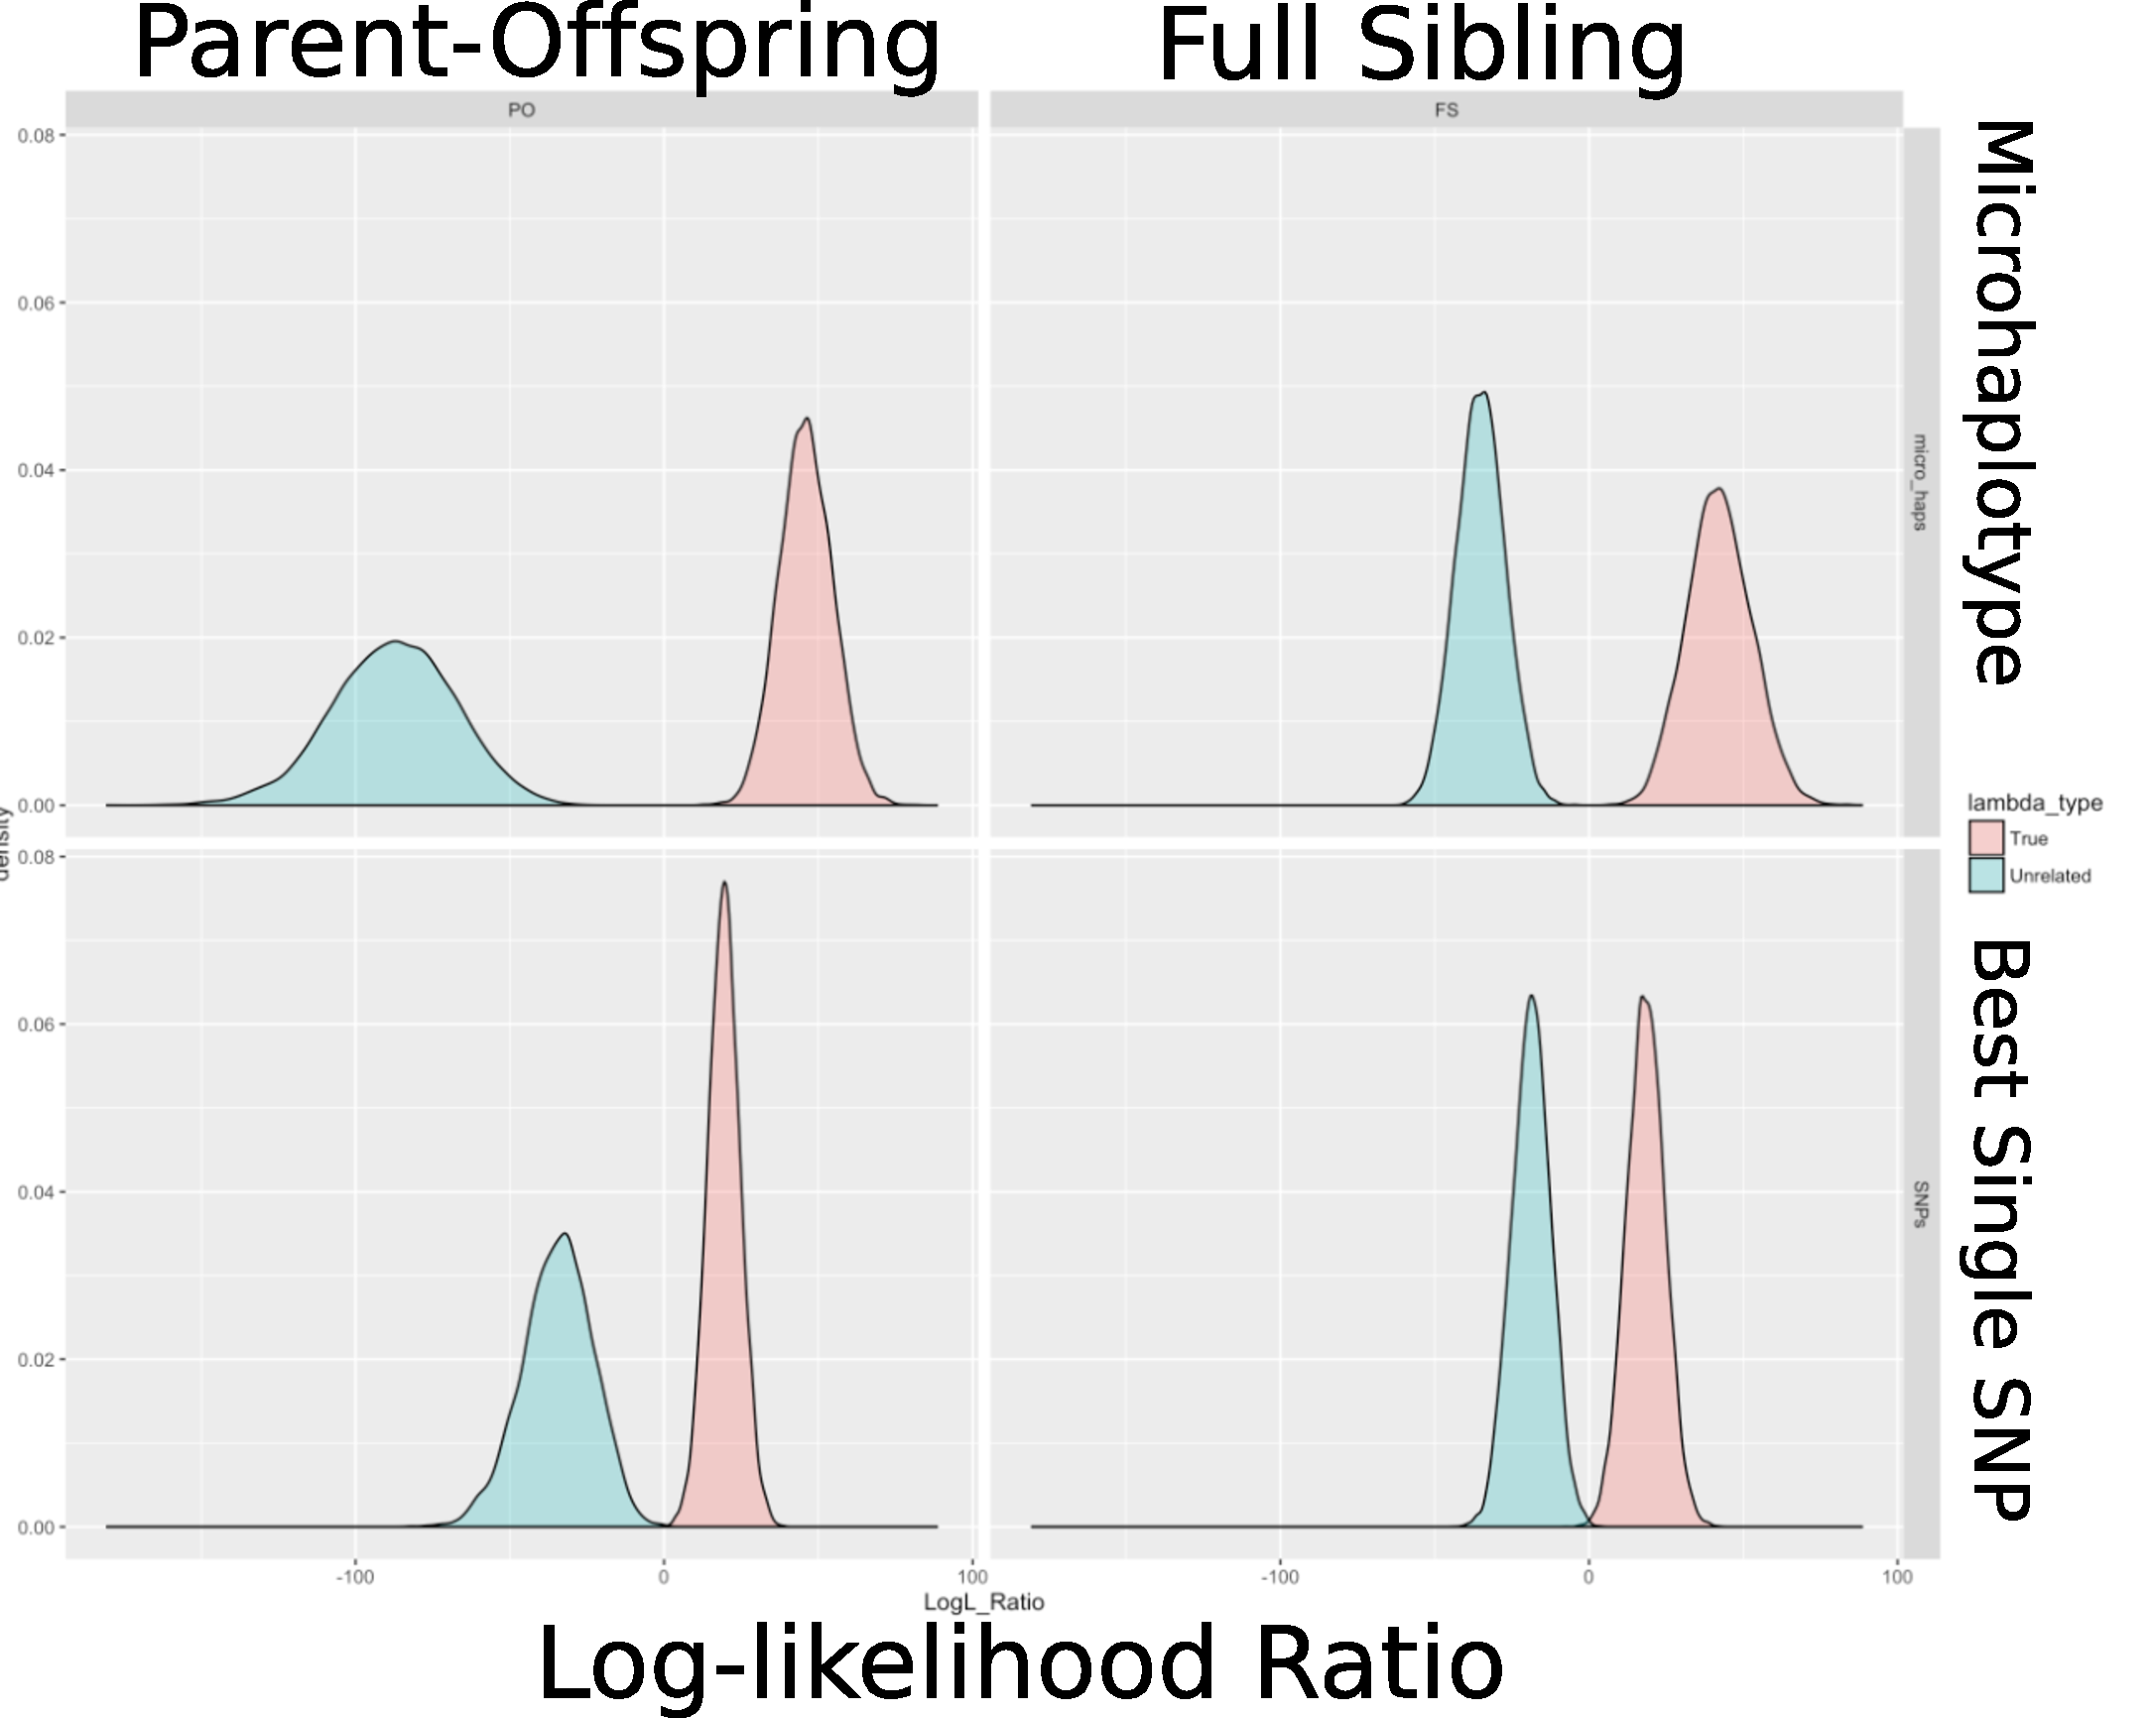
\includegraphics[width = 0.84\textwidth]{mhap_figs/loglrats.pdf}
\end{center}

\end{frame}













\begin{frame}{Log-likelihood ratio distribution}
\framesubtitle{False Positive Rates for Unrelated individuals at False Negative Rate = 1\%}
\begin{center}
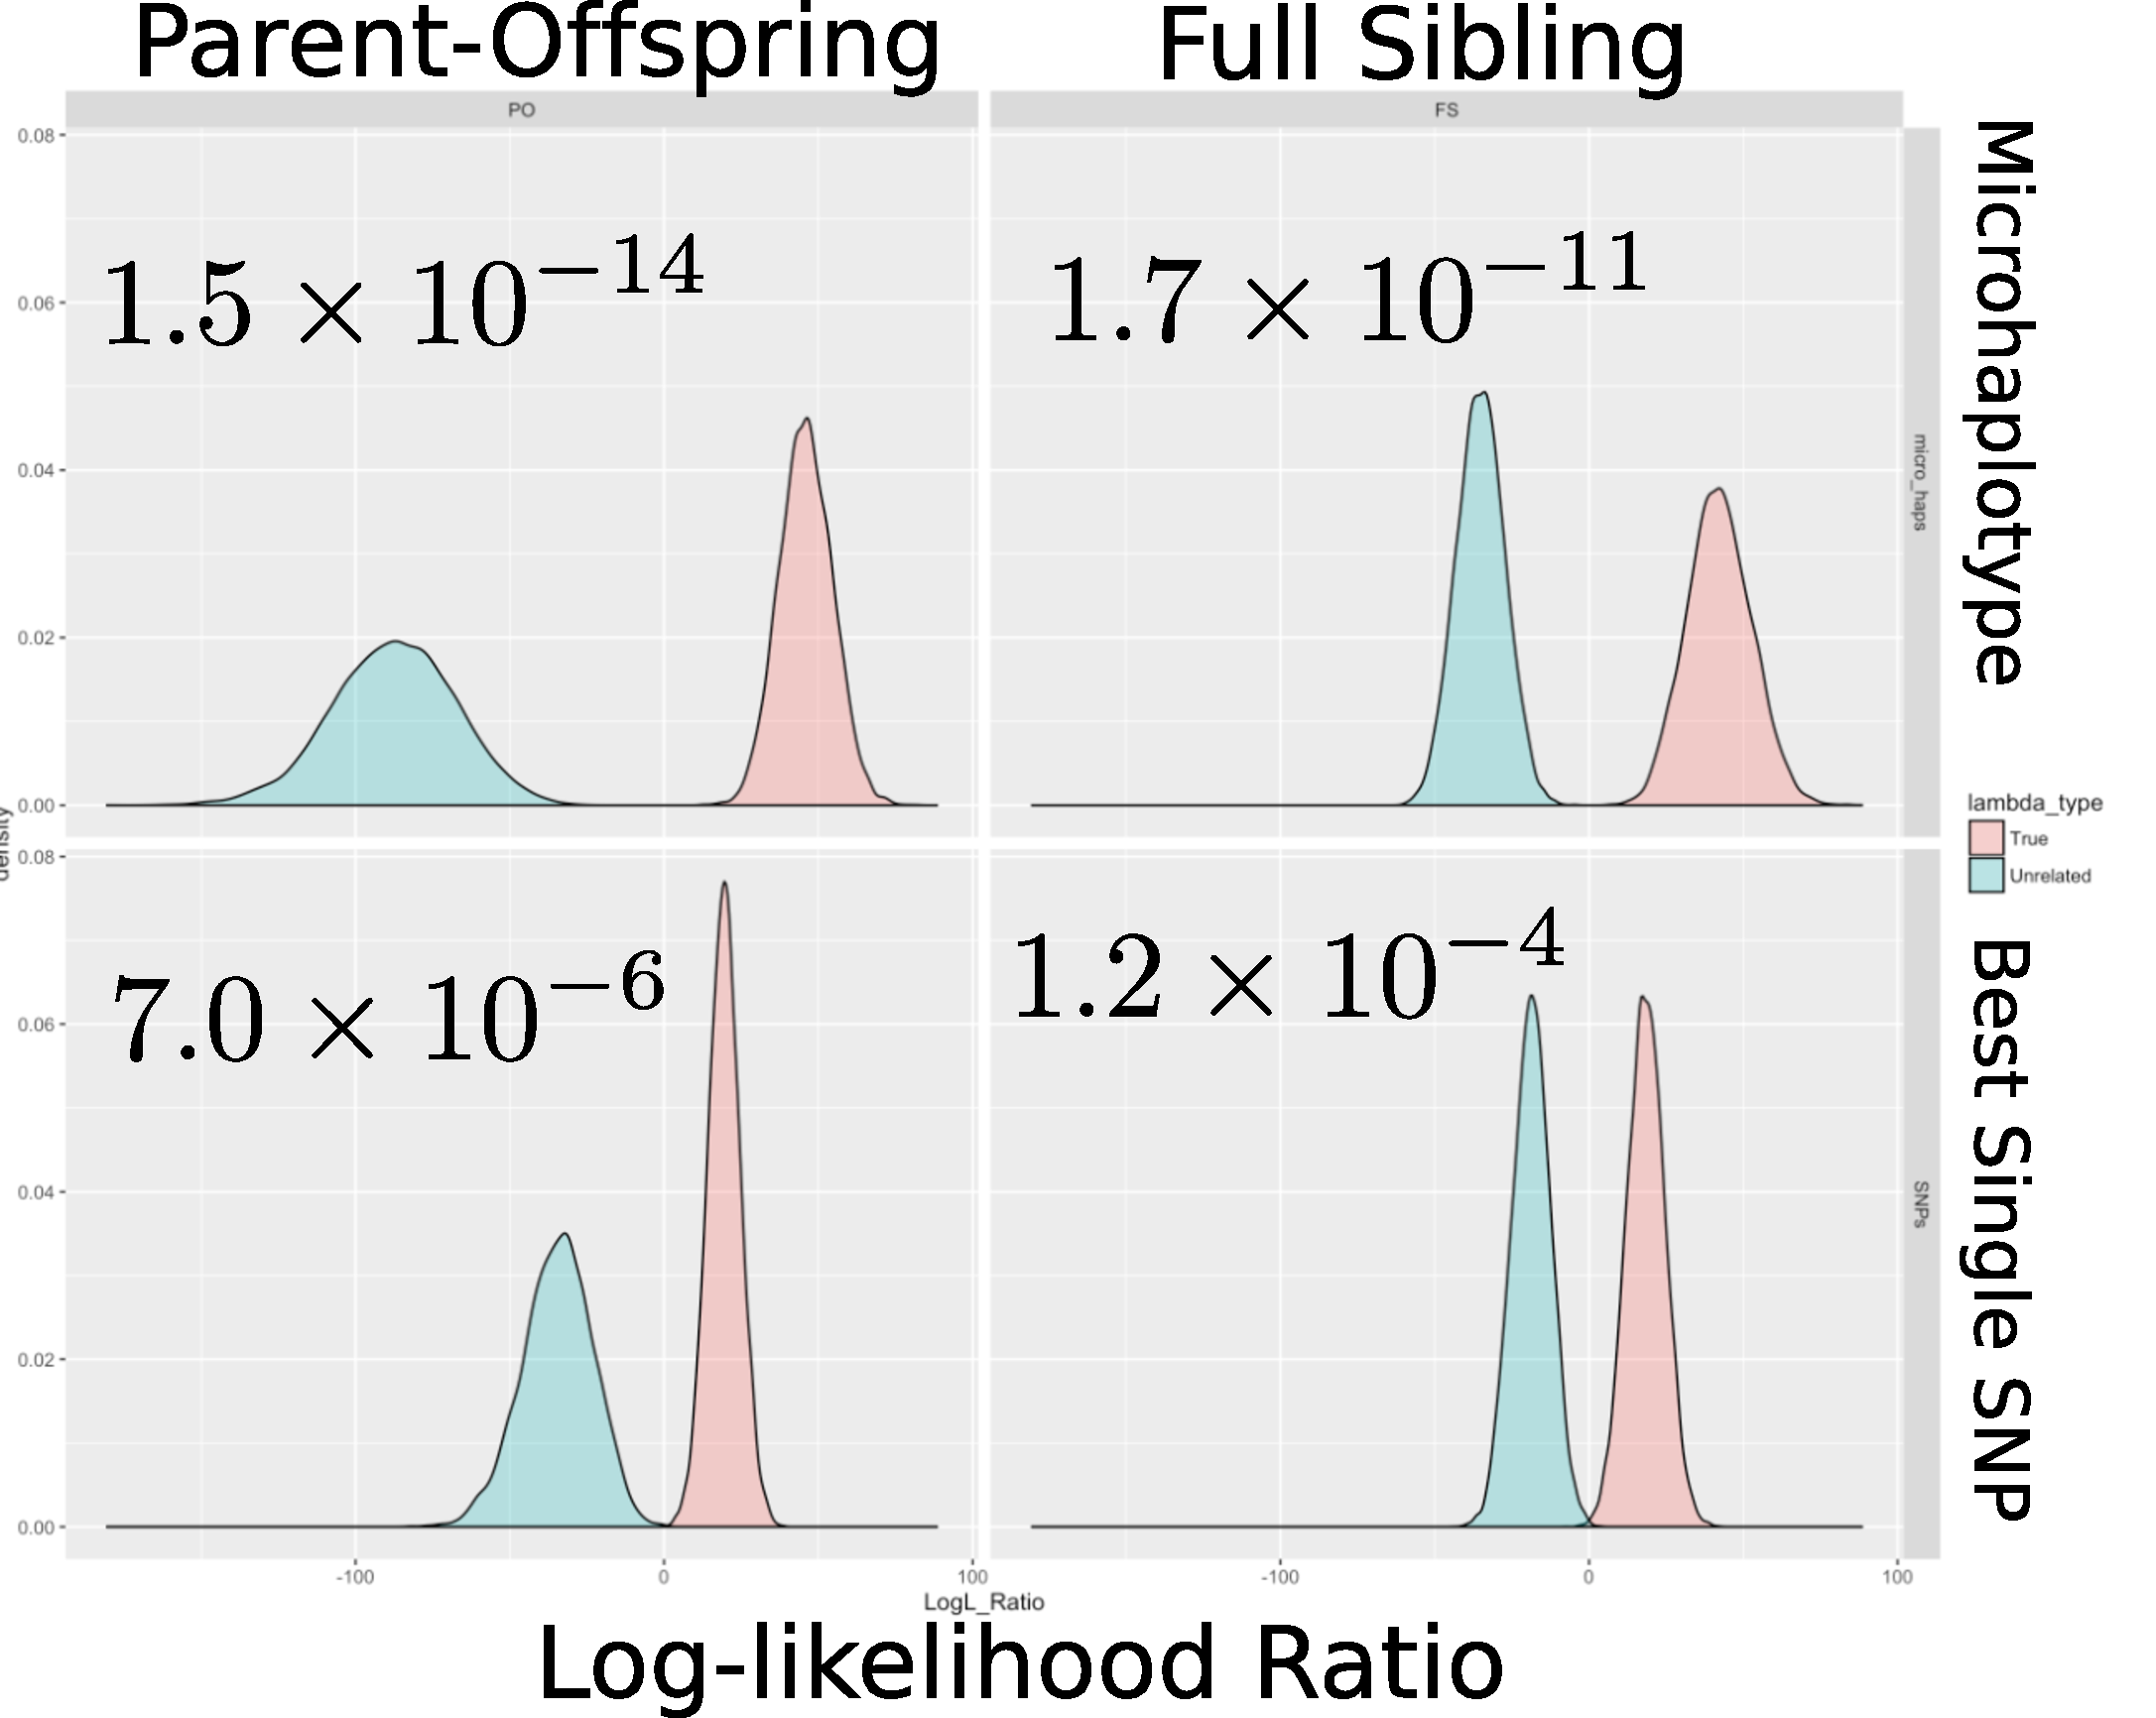
\includegraphics[width = 0.84\textwidth]{mhap_figs/loglrats-FPR.pdf}
\end{center}

\end{frame}












\begin{frame}{Outstanding for Relationship Inference}
\begin{itemize}
\item A false positive rate of $1.5 \times 10^{-14}$ means you could compare 1 million candidate parents to 1 million unrelated candidate offspring and not expect any errors.
\item Using just a single SNP from each locus you would expect 7 errors when comparing 1,000 candidate parents to 1,000 unrelated candidate offspring.
\item Genotyping costs dropping toward $<$\textsterling 5 per sample.
\item Very exciting for ``close-kin mark-recapture''\\
{\em Statistical Science}~31:259--274. (2016)
\end{itemize}
\begin{center}

\includegraphics[width = 0.7\textwidth]{mhap_figs/ckmr-header.png}
\end{center}
\end{frame}







\begin{frame}{Nuts and bolts}
\framesubtitle{Software from our lab -- I}

{\tt\Large haplot}
\begin{itemize}
\item an R package
\item Extract haplotypes from SAM files
\item Filter on Read Depth / Allelic Balance ratio
\item Partially completed Bayesian inference of haplotypes
\item Full Shiny App for Visualization.
\end{itemize}

{\tt https://github.com/ngthomas/haplot}
\end{frame}


\newpage
\mbox{}
\vspace*{2em}
\mbox{}
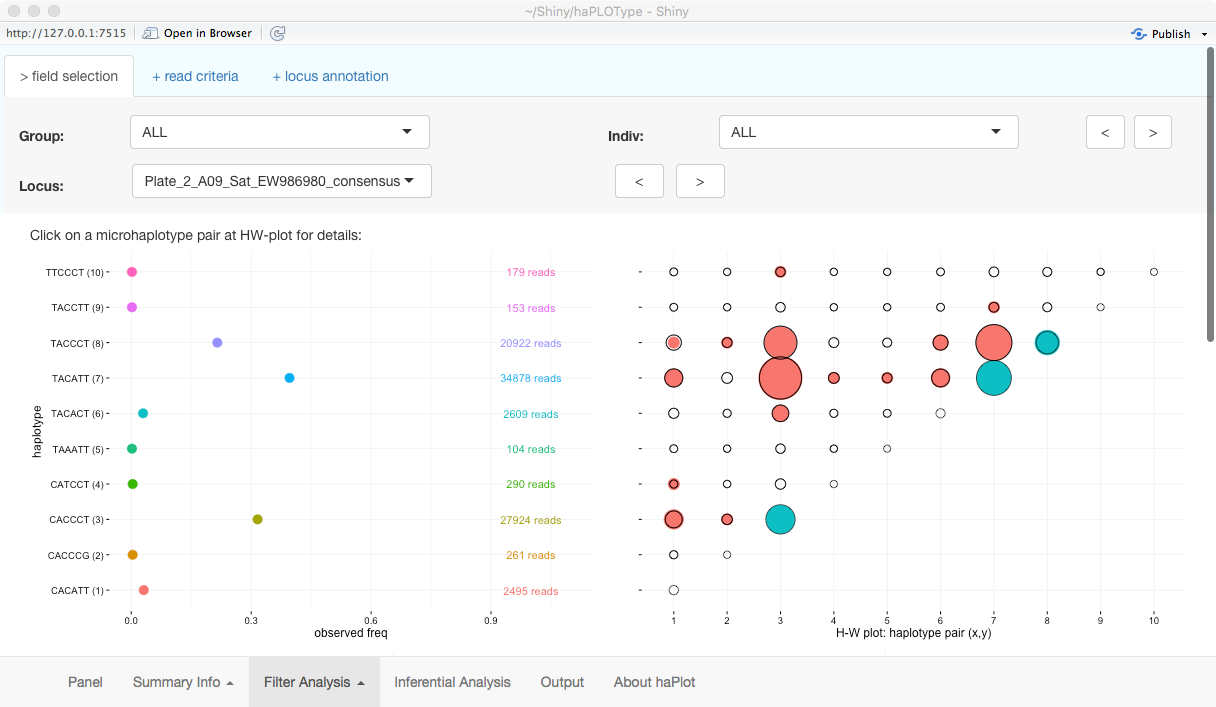
\includegraphics[width=\textwidth]{mhap_figs/haplot2.png}



\begin{frame}{Nuts and bolts}
\framesubtitle{Software from our lab -- II}

{\tt\Large CKMRsim}
\begin{itemize}
\item an R package
\item Estimate false positive rates for pairwise relationship inference
\item Built to accommodate general genotyping error models
\item Importance sampling algorithm to estimate very small probabilities
\item Integration with Mendel to simulate linked markers
\item Key parts written in C++ for speed.
\end{itemize}

{\tt https://github.com/eriqande/CKMRsim}
\end{frame}



\begin{frame}{Conclusions}


This talk available at:
{\tt https://github.com/eriqande/TALKS-microhap}
\end{frame}


\end{document}



